%% Copernicus Publications Manuscript Preparation Template for LaTeX Submissions
%% ---------------------------------
%% This template should be used for copernicus.cls
%% The class file and some style files are bundled in the Copernicus Latex Package, which can be downloaded from the different journal webpages.
%% For further assistance please contact Copernicus Publications at: production@copernicus.org
%% http://publications.copernicus.org/for_authors/manuscript_preparation.html
%% Please use the following documentclass and journal abbreviations for discussion papers and final revised papers.
%% 2-column papers and discussion papers
\documentclass[gmd, manuscript]{copernicus}
%% Journal abbreviations (please use the same for discussion papers and final revised papers)
% Archives Animal Breeding (aab)
% Atmospheric Chemistry and Physics (acp)
% Advances in Geosciences (adgeo)
% Advances in Statistical Climatology, Meteorology and Oceanography (ascmo)
% Annales Geophysicae (angeo)
% ASTRA Proceedings (ap)
% Atmospheric Measurement Techniques (amt)
% Advances in Radio Science (ars)
% Advances in Science and Research (asr)
% Biogeosciences (bg)
% Climate of the Past (cp)
% Drinking Water Engineering and Science (dwes)
% Earth System Dynamics (esd)
% Earth Surface Dynamics (esurf)
% Earth System Science Data (essd)
% Fossil Record (fr)
% Geographica Helvetica (gh)
% Geoscientific Instrumentation, Methods and Data Systems (gi)
% Geoscientific Model Development (gmd)
% Geothermal Energy Science (gtes)
% Hydrology and Earth System Sciences (hess)
% History of Geo- and Space Sciences (hgss)
% Journal of Sensors and Sensor Systems (jsss)
% Mechanical Sciences (ms)
% Natural Hazards and Earth System Sciences (nhess)
% Nonlinear Processes in Geophysics (npg)
% Ocean Science (os)
% Proceedings of the International Association of Hydrological Sciences (piahs)
% Primate Biology (pb)
% Scientific Drilling (sd)
% SOIL (soil)
% Solid Earth (se)
% The Cryosphere (tc)
% Web Ecology (we)
% Wind Energy Science (wes)
%% \usepackage commands included in the copernicus.cls:
%\usepackage[german, english]{babel}
%\usepackage{tabularx}
%\usepackage{cancel}
%\usepackage{multirow}
%\usepackage{supertabular}
%\usepackage{algorithmic}
%\usepackage{algorithm}
%\usepackage{amsthm}
%\usepackage{float}
%\usepackage{subfig}
%\usepackage{rotating}
\begin{document}
%<<<<<<< HEAD

\title{Plume-SPH 1.0: A three-dimensional, dusty-gas volcanic plume model based on smoothed particle hydrodynamics}

%>>>>>>> 0d96d9682fb484b8b159e8d09a0eb89723d3a0f8
% \Author[affil]{given_name}{surname}
\Author[1]{Zhixuan}{Cao}
\Author[1]{Abani}{Patra}
\Author[2]{Marcus}{Bursik}
\Author[3]{E. Bruce}{Pitman}
\Author[4]{Matthew}{Jones}
\affil[1]{Department of Mechanical and Aerospace Engineering and Computational Data Science and Engineering, University at Buffalo, SUNY, New York, USA}
\affil[2]{Department of Geology, University at Buffalo, SUNY, New York, USA}
\affil[3]{Department of Material Design and Innovation, University at Buffalo, SUNY, New York, USA}
\affil[4]{Center for Computational Research,
University at Buffalo, SUNY, New York, USA}
%% The [] brackets identify the author with the corresponding affiliation. 1, 2, 3, etc. should be inserted.
\runningtitle{Plume-SPH 1.0}
\runningauthor{Z. Cao et al}
%<<<<<<< HEAD
\correspondence{Abani Patra (abani@buffalo.edu)}
%=======
%\correspondence{Abani Patra (abani.patra@gmail.com)}
%>>>>>>> 0d96d9682fb484b8b159e8d09a0eb89723d3a0f8
\received{}
\pubdiscuss{} %% only important for two-stage journals
\revised{}
\accepted{}
\published{}
%% These dates will be inserted by Copernicus Publications during the typesetting process.
\firstpage{1}
\maketitle
\begin{abstract}

Plume-SPH provides the first particle based simulation of volcanic plumes. SPH (smoothed particle hydrodynamics) has several advantages over currently used mesh based methods in modeling of multiphase free boundary flows like volcanic plumes. This tool will provide more accurate eruption source terms to users of VATDs (Volcanic ash transport and dispersion models) greatly improving volcanic ash forecasts. The accuracy of these terms is crucial for forecasts from VATDs and the 3D SPH model presented here will provide better numerical accuracy. As an initial effort to exploit the feasibility and advantages of SPH in volcanic plume modeling, we adopt a relatively simple physics model (3D dusty-gas dynamic model assuming well mixed eruption material, dynamic equilibrium and thermodynamic equilibrium between erupted material and air that entrained into the plume, and minimal effect of winds) targeted at capturing the salient features of a volcanic plume. The documented open source code is easily obtained and extended to incorporate other models of physics of interest to the large community of researchers investigating multiphase free boundary flows of volcanic or other origins. 

The Plume-SPH code also incorporates  several newly developed techniques in SPH  needed to address numerical challenges in simulating multiphase compressible turbulent flow. The code should thus be also of general interest to the much larger community of researchers using and developing SPH based tools. In particular, the $SPH-\varepsilon$ turbulence model is to capture mixing at unresolved scales. Heat exchange due to turbulence is calculated by a Reynolds analogy and a corrected SPH is used to handle tensile instability and deficiency of particle distribution near the boundaries. We also developed methodology to impose velocity inlet and pressure outlet boundary conditions, both of which are scarce in traditional implementations of SPH.

The core solver of our model is parallelized with MPI (message passing interface) obtaining good weak and strong scalability using novel techniques for data management using a SFCs (space-filling curves) and object creation time based indexing and hash table based storage scheme. These techniques are of interest to researchers engaged in developing particle in cell type methods. The code is first verified by 1D shock tube tests, then by comparing velocity and concentration distribution along the central axis and on the transverse
cross with experimental results of JPUE (jet or plume that is ejected from a nozzle into a uniform environment). 
%The model is validated by comparing against simulation results from other 3D plume models.
Profiles of several integrated variables are compared with those calculated by existing 3D plume models for an eruption with the same MER (mass eruption rate) estimated for the Pinatubo eruption of June 15 1991. Our results are consistent with existing 3D plume models. Analysis of the plume evolution process demonstrates that this model is able to reproduce the physics of plume development. 

\end{abstract}

\introduction  %% \introduction[modified heading if necessary]
%<<<<<<< HEAD
\subsection{Volcanic ash hazards}
Primary hazards associated with explosive volcanic eruptions include pyroclastic density currents (flows and surges), the widespread deposition of airfall tephra, and the threats to aviation posed by volcanic ash in the atmosphere.
Simulation of all possible hazards with one model is difficult due to the fact that different length scales dominate different hazards. Our focus here is the hazard that volcanic ash poses to aircraft. 

During volcanic eruptions, VATDs (volcanic ash transport and dispersion models) are used to forecast the location and movement of ash clouds at timescales that range from hours to days. VATDs use eruption source parameters, such as plume height, mass eruption rate, duration, and the mass fraction distribution of erupted particles finer than about $4 \Phi$ (or $62.5 \mu$m), which can remain in the cloud for many hours or days. Observational data for such parameters are usually unavailable in the first minutes or hours after an eruption is detected. Moreover, these input parameters are subject to change during an eruption, requiring rapid re-assignment of new parameters. Usually, plume models are used to provide these source terms for VATDs and the forecast accuracy is critically dependent on these models. This paper reports on a new 3D (three dimensional) volcanic plume model designed to exploit the advantages of mesh-free methods for 3D modeling of such plumes that involve multiphase free boundary flows.

%The dynamics of explosive eruption clouds has been a central issue of volcanology science for a long time \citep{settle1978volcanic, wilson1978control}.
%The basic physics of volcanic plumes has been studied for more than half a century \citep{morton1956turbulent, settle1978volcanic, wilson1978control}. The effects of magma type and vent conditions \citep{woods1988fluid, woods1995decompression}, atmospheric conditions \citep{ woods1993moist, sparks1997volcanic, bursik2001effect}, external surface water \citep{koyaguchi1996formation}, thermal disequilibrium, and particle fallout \citep{woods1991particle} have been assessed in increasing details based on observation, experiments and numerical studies.

\subsection{Existing plume models}
Several 1D (one dimensional) volcanic plume models have been developed in the past few decades, ranging from the most basic 1D model \citep{woods1988fluid} which only accounts for mass conservation to more recently developed 1D models  \citep{bursik2001effect, mastin2007user, degruyter2012improving, woodhouse2013interaction, devenish2013using, de2015plume, folch2016fplume, pouget2016sensitivity} which tend to account for more comprehensive physics effects. 
For example, FPLUME-1.0 \citep{folch2016fplume} accounts for wind effect, entrainment of moisture, water phase change, particle fallout and re-entrainment and even wet aggregation of ash. However, in these 1D models, the entrainment of air is evaluated based on two coefficients: entrainment coefficient due to turbulence in the rising buoyant jet and the crosswind field. Different 1D models adopt different entrainment coefficients based on specific formulation or calibration against well-documented case studies. The feedback from plume to atmosphere is usually ignored in 1D models. Even though determination of essential parameters such as the entrainment is not based on first principles, such simple models nevertheless allow us to investigate the importance of physical mechanisms in a volcanic plume. In addition, these simplified models require little computational resource and can run on standard personal computers or on web sites in very short time. As a result, 1D software for volcanic plume development \citep[such as][]{267, 1194, 3541}, combined with VATDs \citep[such as][]{114, draxler2015hysplit} are widely used in research and practice. While these 1D models can generate well-matched results with 3D (three dimensional) models for weak plumes, much greater variability is observed for strong plume scenarios, especially for local variables \citep{costa2016results}. In addition, there is need for greater skill in hazards forecasts especially where the plume model is used to generate source conditions for complex 2D (two dimensional) and 3D VATD models.

The development of 2D and 3D, time-dependent, and multiphase numerical models for volcanic plumes has provided new explanations for many features of explosive volcanism. For example, a recent study based on 3D fluid dynamical model \citep{costa2018understanding} shows that simple extrapolations of integral models for Plinian columns to those of super-eruption plumes are not valid and their dynamics diverge from current ideas of how volcanic plumes operate. One of the earliest of these is the 3D model PDAC (Pyroclastic Dispersion Analysis Code) \citep{neri2003multiparticle}  which is a non-equilibrium, multiphase, 3D compressible flow model. Conservation equations for each phase are solved separately with the finite volume method. A parallel computing version of PDAC was also developed \citep{ongaro2007parallel}. Advanced numerical techniques, such as a second order scheme and semi-explicit time stepping, was also adopted afterwards to improve the accuracy of PDAC \citep{carcano2013semi}. 

Another 3D model, SK-3D \citep{suzuki2005numerical} is a 3D time-dependent fluid dynamics model that attempts to reproduce the entrainment process of eruption clouds with relatively simple physics but with high order numerical accuracy and high spatial resolution.
A series of simulations based on SK-3D was reported, including establishment of the relationship between the observable quantities of the eruption clouds and the eruption conditions at the vent \citep{suzuki2009three}, investigation of the effect of the intensity of turbulence in the umbrella cloud on dispersion and sedimentation of tephra \citep{koyaguchi2009effect}, determination of the entrainment coefficients of eruption columns as a function of height \citep{suzuki2010numerical} and investigation of the effect of wind field on entrainment coefficient \citep{suzuki20133d}. 

While SK-3D focuses on accurately capturing the entrainment caused by turbulent mixture with higher resolution and numerical method of higher order, PDAC takes the disequilibrium between different phases into account and hence is a true multiphase model. Another 3D model, ATHAM (Active Tracer High-Resolution Atmospheric Model) \citep{oberhuber1998volcanic} focuses more on microphysics within the plume. As pyroclastic flow is not the initial concern of ATHAM, dynamic and thermodynamical equilibrium is assumed in ATHAM. The dynamic core of ATHAM solves the compressible Euler equations for momentum, pressure and temperature of the gas particle mixture \citep{oberhuber1998volcanic}. The subgrid-scale turbulence closure scheme that differentiates between the horizontal and vertical directions \citep{herzog2003prognostic} is adopted to capture turbulent mixing. The cloud microphysics predicts the mass of hydrometeors in liquid and ice phase \citep{herzog1998effect}. Additional modules, including gas phase chemistry \citep{trentmann2002simulation} and gas scavenging by hydrometeors \citep{textor2003injection} were added lately. A further extension was made to include particle aggregation \citep{textor2006volcanic1, textor2006volcanic2}. However, the resolution of ATHAM is still coarse compared with SK-3D and PDAC.

Besides adding to their special strengths (ATHAM has been adding more and more microphysics, PDAC was extended to consider more phases), these models are also adding core strengths. PDAC development has begun to include the effect of microphysics into the model while ATHAM development has extended its ability to modeling pyroclastic flow. Both are using finer and finer resolution. 

Recently, a first order, nonequilibrium compressible 3D model, ASHEE \citep{cerminara2016ashee}, was introduced based on three dimensional N-phases Eulerian transportation equations, which are a full set of mass, momentum and energy transport equations for a mixture of gas and dispersed particles. ASHEE is valid for low concentration and low Stokes number region and much faster than N-phases Eulerian model. The model is based on the open source numerical solver OpenFOAM \citep{weller1998tensorial}, adapting its unstructured finite volume solver.

To summarize, each 3D model has its own focus based on the problem of interest and modeling/numerical choices made.
 %Different simplification was made based on their scope. Improvements have been making since their birth. 
 Accuracy of simulation (depending on comprehensiveness of the model, resolution of discretization, numerical error, and order of accuracy) and simulation time (depending on number of governing equations, resolution, numerical methods and parallel techniques) are always conflicting considerations in 3D plume simulations.

\subsection{Features of SPH}
To the best of our knowledge, all of the existing 3D plume models use mesh based Eulerian methods, and there are no 3D plume models based on mesh free Lagrangian methods. Lagrangian methods have several features that are suitable for volcanic plume simulation that we outline below. Among such Lagrangian methods, smoothed particle hydrodynamics \citep{gingold1977smoothed,lucy1977numerical} based simulations have shown good agreement with experiments for many applications in fluid dynamics. Currently it is, by far, the most widely used mesh-free scheme. Our implementations of SPH in volcanology follows on earlier efforts   \citep{bursik2003smoothed,herault2010sph,haddad2016smoothed}.
Specifically, we choose SPH as the numerical method for volcanic plume simulation to enable:
\begin{itemize}
\item better investigation of mixing phenomena;
\item accurate modeling of the development of ZFE (Zone of Flow Establishment), ZEF (Zone of Established Flow) investigation and relation to column collapse and the questions relating to the development of entrainment;
\item  easy inclusion of particles of different sizes (phases) and investigation of detailed mechanics of sedimentation and drag force interaction in lower plume.
\end{itemize}

These are enabled by the following features of SPH:
\begin{itemize}
%\item For mesh based method, either interface tracking (Lagrangian) \citep{harlow1965numerical, wrobel1991computational, cheng1995simplified} or interface capturing (Eulerian) \citep{hirt1981volume, youngs1982time, gerlach2006comparison, gopala2008volume} methods are used to reconstruct the flow interface of free boundary flow. High computational cost, a tendency to form numerical instabilities and the inability to track complex topological changes are the significant drawbacks of tracking techniques \citep{hirt1981volume, unverdi1992front, anderson1998diffuse}. For interface capturing (Eulerian) method, the surrendering of surface detail before the phase transport calculation means that interface reconstruction is required between time steps to recover the interface information, which needs additional numerical effort \citep{hirt1981volume, youngs1982time}. Since SPH is able to adaptively adjust the discretization and automatically construct the interface, SPH does not require additional numerical effort for interface construction and therefore is more suitable for volcanic plume simulation.
\item Advection term in the Navier-Stokes equations does not appear explicitly in discretized formula of SPH (as illustrated in Eq. (\ref{eq:gov-nc-rho}) to Eq. (\ref{eq:gov-nc-e})).
\item It is easy to include various physics effects (like self gravity, radiative cooling and chemical reaction) into the model. It does not require a major overhaul and re-tooling every time new physics is introduced \citep{monaghan1995sph}. This implies that accounting for more physics is easier for SPH model.
\item With more than one phase, each described by its own set of particles, interface problems between phases are often trivial for SPH but difficult for mesh based schemes. So multiphase flow can be easily handled by SPH. Adding of new phases to the model also does not require a major overhaul and re-tooling. As will be shown in later paragraphs, adding of new phases only leads to adding of several lines into the source code for new phases and additional interaction terms between existing phases and newly added phases.
\item Interface tracking is explicit in SPH through capturing of the locations of the particles. Less numerical effort is required for interface construction when we attempt to include the effects of mixing by resolving the detailed interface structure and dynamics of turbulence.
\end{itemize}

As discussed in the previous paragraph, existing 3D plume models focus on one or several specific aspects of plume and have been extended to be more comprehensive by accounting for more physics or more phases. Easy extensibility and capability of handling multiple phase flow with less additional numerical effort greatly facilitate future extension of SPH models. As volcanic plumes are in nature multiphase and without pre-defined boundary in the atmosphere, SPH is a suitable numerical method for plume modeling. The core physics, such as entrainment of air and thermal expansion, are essential for all plume modeling while some other physics, such as water condensation and aggregation etc., are important in specific scenarios. As an initial effort on exploiting advantages of SPH in volcanic plume modeling, we focus on capturing basic features in plume development using a numerically robust and computationally efficient framework with support for scalable parallel computing. %So our current model is far away from comprehensive. 

Open source availability and the relatively easy extensibility of SPH will facilitate development of a more comprehensive community driven model.

\subsection{Our contributions}
Even though SPH has been known for several decades, implementations of SPH for compressible multiphase turbulent flows are few. \citet{colagrossi2003numerical} proposed a multiphase SPH model for numerical simulation of air entrapment in violent fluid-structure interactions. \citet{hu2007incompressible} and \citet{adami2010new} proposed weakly compressible and incompressible multiphase SPH solvers in their papers. \citet{monaghan2013simple} also proposed new formulations for weakly compressible fluid with speed of sound sufficiently large to guarantee that the relative density variations are typically $1\%$. \citet {chen2015sph} recently presented a new SPH model for weakly compressible multiphase flows with complex interfaces and large density differences. All of them focus on incompressible or weakly compressible flow.

Several issues endemic to classical SPH, like tensile instabilities,  compressible turbulence modeling and turbulent heat exchange, are fixed in our implementation. The most popular applications of SPH (and their original motivating application) has been in the simulation of free surface flow, such as breaking-waves and floods. Less attention was paid to velocity inlet and pressure outlet boundary conditions which are required in plume modeling.
 
\begin{itemize}
\item We develop methodology to impose pressure boundary conditions by adding extra layers of static ghost particles. Additional constraints on the time step are used to avoid the growth of numerical fluctuations near the pressure boundary. We impose a velocity inlet boundary condition by placing several layers of ghost particles moving with eruption velocity. 
\item Turbulence model is crucial for reproducing the entrainment of air. There are several turbulence models proposed for SPH method \citep{issa2005numerical,violeau2007numerical}. We adopt a LANS (Lagrangian Averaged Navier-Stokes) turbulence model \citep{monaghan2011turbulence}, which was originally proposed for incompressible flow, and is extended here for compressible flow accounting for turbulent heat exchange. 
\item Corrected formulation of SPH \citep{chen1999improvement} is adopted to bypass the well-known tensile instability issues of classical SPH.
\item Simulation of volcanic plumes with acceptable accuracy requires fine resolution (very high particle counts) that cannot be accomplished without parallel computing using large process counts. The core solver of our model is parallelized by distributed memory MPI (message passing interface standard) parallelism. In addition, a dynamic load balancing strategy is also developed. 
\item Imposition of some types of boundary conditions (such as eruption boundary condition) requires dynamically adding and removing of particles during simulation. To address this issue, we adopt an efficient data management scheme based on time dependent SFC (space filling curve) induced indexing and hash table. The computational cost is further reduced by adjusting simulation domain adaptively.
\end{itemize}

The physical model of the plume is first presented in section \ref{sec:physics-model} and leads to a complete mathematical description of the volcanic plume (governing equations and boundary conditions). In section \ref{sec:SPH_method}, we  briefly introduce the numerical tool -- the SPH method. Both the fundamental discretization formulation and techniques that are used to handle specific issues involved in plume modeling are discussed. Verification and validation with numerical tests are presented in section \ref{sec:verification-validation}. In section \ref{sec:conclusion}, a discussion on future work is given following a brief summary.

\section{Physical model} \label{sec:physics-model}
\subsection{Description of the model}
During an explosive eruption, a volcanic jet erupts out from a vent with a speed of several tens to more than 150 meters per second, driven by expanding gas. The jet is initially denser than the surrounding atmosphere and begins to decelerate through negative buoyancy and turbulent interaction with surrounding air. Cauliflower-like vortices are generated along jet margins, within which process, air is entrained and heated up, reducing the bulk density of the entire jet, in many cases, to less than that of the surrounding atmosphere. Once it becomes buoyant, such a jet develops into a plinian or subplinian plume, rising up to several kilometers to tens of kilometers until its heat is exhausted. Jets that lose their momentum before becoming buoyant collapse back onto the ground and transform into pyroclastic flows, surges and ignimbrites. During the process of plume rising up, relatively larger particles might separate from main stream of the plume, falling down onto the ground and possibly be re-entrained into the plume at a lower height \citep{ernst1996sedimentation}. Within this process, erupted vapor condenses to liquid (droplet) and even further to ice. Latent heat released from phase change of erupted vapor  further heats up entrained air and further dilutes the bulk density. The entrained vapor might also experience a similar process and impact plume development. Particle aggregation processes \citep{carey1982influence,taddeucci2011aggregation}, either due to presence of liquid water, resulting from particle collision or driven by electrostatic forces might occur inside plume and thereby affect the sedimentation. 

All in all, the process of plume development is  essentially a multiphase turbulent mixing process coupled with heat transfer and other microphysical and chemical reactions.

As an initial effort on exploiting the feasibility and advantage of SPH in plume modeling, our model is designed to describe an injection of well mixed solid and volcanic gas from a circular vent above a flat surface into a stratified stationary atmosphere following SK-3D \citep{suzuki2005numerical}. In this model, molecular viscosity and heat conduction is neglected since turbulent exchange coefficients are dominant. Erupted material consisting of solid with different size and mixture of gases is assumed to be well mixed and behave like a single phase fluid (phase 2) which is valid for eruptions with fine particles and ash. Air (also a mixture of different gases) is assumed to be another phase (phase 1). Thermodynamic equilibrium is assumed so that no separate energy equation is needed for each phase. As a result, there is only one energy equation for both phases (heat exchange term between different phases does not show up under this assumption). Dynamic equilibrium is assumed so that no separate momentum equation is needed for each phase. As a result, there is only one vector momentum equation for both phases (drag force term does not show up with this assumption). 

Because of the above assumptions, all other microphysical processes (such as the phase changes of \texorpdfstring{H\textsubscript{2}O}, aggregation, disaggregation, absorption of gas on the surface of solids, solution of gas into a liquid) and chemical processes are not considered in this model. These ignored microphysics factors would play critical roles under particular eruption conditions. Capturing of these processes needs a more comprehensive model. One critical element in plume development, the effect of wind, is also not yet considered in this model. Introducing wind effects in our model requires dynamic pressure boundary conditions, which requires more numerical effort and algorithm design. To summarize, our model is not valid for eruptions where wind effect plays a significant role in its development, usually refered as a weak plume. Our model also lacks the ability in modeling plumes with large particles or eruptions in which microphysics plays non-ignorable roles, such as an eruption of \textit{El Chich{\'o}n} volcano on April 4th 1982 \citep{sigurdsson19841982, folch2016fplume}. We are focussed here on developing the SPH based methodoloy in the context of the more basic (and more critical) aspects of volcanic plume and therefore devote our effort to this relative simpler model. It is worthwhile to mention here that because SPH is adopted as our numerical method, adding of these physics into our model would require much less work in terms of programming compared to mesh based methods. Since our plan is an open source distribution of the tool we believe some of these enhancements will rapidly ensue with community participation.

\subsection{Governing equations}
Based on above assumptions, the governing equations of our model are given as (which is the same as the governing equations of SK-3D \citep{suzuki2005numerical}):
\begin{align}
\dfrac{\partial \rho}{\partial t} + \nabla \cdot \left(\rho \textbf{v}\right) = 0 \label{eq:gov-cs-rho} \\
\dfrac{\partial \rho \xi}{\partial t} + \nabla \cdot \left(\rho \xi \textbf{v}\right) = 0 \label{eq:gov-cs-ks}\\
\dfrac{\partial \rho \textbf{v}}{\partial t} + \nabla \cdot \left(\rho \textbf{v} \textbf{v} + p\textbf{I}\right) = \rho \textbf{g} \label{eq:gov-cs-v} \\
\dfrac{\partial \rho E}{\partial t} + \nabla \cdot \left[\left(\rho E + p \right)\textbf{v}\right] = \rho \textbf{g} \cdot\textbf{v} \label{eq:gov-cs-e}
\end{align}
where $\rho$ is the density, $\textbf{v}$ is the velocity, $\xi$ is the mass fraction of ejected material, $\textbf{g}$ is the gravitational acceleration, $\textbf{I}$ is a unit tensor.
$E = e + K $ is the total energy which is a summation of kinetic energy $K$ and internal energy $e$.
An additional equation is required to close the system. In this model, the equation for closing the system is the following EOS (equation of state).
\begin{equation}
p = \left(\gamma_m - 1\right)\rho e \label{eq:EOS}
\end{equation}
where 
\begin{equation}
\gamma_m = R_m/C_{vm} + 1 \label{eq:gov-gm}
\end{equation}
\begin{equation}
R_m = \xi_g R_g + \xi_a R_a  \label{eq:gov-Rm}
\end{equation}
\begin{equation}
C_{vm} = \xi_s C_{vs} + \xi_g C_{vg} + \xi_a C_{va} \label{eq:gov-Cvm}
\end{equation}
\begin{equation}
\xi_a = 1 - \xi \label{eq:gov-na}
\end{equation}
\begin{equation}
\xi_g = \xi \cdot \xi_{g0} \label{eq:gov-ng}
\end{equation}
\begin{equation}
\xi_s = \xi - \xi_g \label{eq:gov-ns}
\end{equation}
where, $C_v$ is the specific heat with constant volume, $R$ is the gas constant. $\xi$ is the mass fraction of erupted material. The subscript $m$ represents mixture of ejected material and air, $s$ represents solid portion in the ejected material, $g$ represents gas portion in the ejected material, $a$ represents air, $0$ represents phyiscal properties of erupted material. $\xi_{g0}$ is the mass fraction of vapor in the erupted material.

In mesh based methods, governing equations in Eulerian form, Eq. (\ref{eq:gov-cs-rho}) to Eq. (\ref{eq:gov-cs-e}), are directly discretized. For SPH, governing equations in Lagrange form are needed. By deducting kinetic energy from energy equation, subtracting mass conservation from momentum equation, combining transient term and advection term into material derivative term (For any function $A$, material derivative is defined as $\frac{D A}{Dt} = \frac{\partial A}{\partial t} + \textbf{v} \cdot \nabla A$), the governing equations are put into the final form, in which advection term does not appear explicitly.
\begin{align}
\dfrac{D \rho}{D t} + \rho \nabla \cdot \textbf{v} = 0 \label{eq:gov-nc-rho}\\
\dfrac{D \rho \xi}{D t} + \rho \xi \nabla \cdot \textbf{v} = 0 \label{eq:gov-nc-ks}\\
\dfrac{D \textbf{v}}{D t} + \dfrac{\nabla P}{\rho} =\textbf{g} \label{eq:gov-nc-v}\\
\dfrac{D e}{D t} + \dfrac{P \nabla \cdot \textbf{v}}{\rho} = 0 \label{eq:gov-nc-e}
\end{align}
%Governing equations in Lagrangian form, Eq. (\ref{eq:gov-nc-rho}) to Eq.(\ref{eq:gov-nc-e}), and Eulerian form, Eq. (\ref{eq:gov-cs-rho}) to Eq. (\ref{eq:gov-cs-e}), are a\dfrac{•}{•}ly equivalent, as deriving the Lagrangian form from the Eulerian is purely based on mathematics without any additional physical assumptions.

\subsection{Boundary conditions}
In the current model the initial domain is a box. The boundaries are categorized as the velocity inlet (a circular area at the center of the bottom of the box), wall boundary (box bottom) and pressure outlet (other faces of the box).
%probably should add a section to list the input parameters in the verification section

\subsubsection{Velocity inlet}
At the vent, temperature of erupted material $T$, eruption velocity $\textbf{v}$, the mass fraction of vapor in erupted material $\xi_{g0}$ and mass discharge rate $\dot M$ are given. The pressure of erupted material $p$ is assumed to be the same as ambient pressure for pressure-balanced eruption. The radius of vent is determined from $\rho$, $\dot M$ and $\textbf{v}$. Equation (\ref{eq:erupt_bc_rho}) to (\ref{eq:erupt_bc_e}) gives velocity inlet boundary condition wrote in terms of primitive variables.
\begin{align}
\rho =const = p/\left(R_m T\right) \label{eq:erupt_bc_rho} \\
\xi=const=1 \label{eq:erupt_bc_xi}\\
\textbf{v} = const =\{u,v,w\}^T \label{eq:erupt_bc_v}\\
\dfrac{\partial e}{\partial n}=\dot M e_0 /\left(\pi r^2\right) \label{eq:erupt_bc_e}
\end{align} 
where $r$ is the radius of the vent, $n$ is the direction normal to the boundary, $e_0$ is specific internal energy of erupted material which can be calculated based on temperature and specific heat of erupted material.

\subsubsection{Non-slip wall boundary}
Velocity is zero for non-slip wall boundary. If we assume the boundary to be adiabatic, heat flux should be zero on the boundary. The flux of mass should also be zero. As a result, internal energy flux, which consists of heat flux and energy flux carried by mass flux, vanishes on the wall boundary. Equation (\ref{eq:wall_bc_rho}) to (\ref{eq:wall_bc_e}) gives no-slip wall boundary condition written in terms of primitive variables.
\begin{align}
\dfrac{\partial \rho}{\partial n} = const = 0\label{eq:wall_bc_rho} \\
\dfrac{\partial \xi}{\partial n} = const = 0 \label{eq:wall_bc_xi}\\ 
\textbf{v} = const =\{0,0,0\}^T \label{eq:wall_bc_v}\\
\dfrac{\partial e }{\partial n} = 0\label{eq:wall_bc_e}
\end{align} 

\subsubsection{Open outlet pressure boundary condition}
The pressure of the surrounding atmosphere is given. Except for the pressure, boundary values for density, velocity, and energy on the outlet should depend on the solution. As we ignore the viscosity, the shear stress is ignored and normal stress (whose magnitude equals to pressure) balances the ambient pressure.
\begin{equation}
p = p_a\left(z\right)  \label{eq:pressure_bc_p} 
\end{equation} 

\section{SPH method} \label{sec:SPH_method}
SPH is a mesh-free Lagragian method. In SPH, the domain is discretized by a set of particles or discretization points and the position of each particle is updated at every time step based on the motion computed. Approximation of all field variables (velocity, density and pressure, ect.) is obtained by interpolation based on discretization points. The physical laws (such as conservation laws of mass, momentum and energy) written in the form of PDEs (partial differential equations)  or ODEs (ordinary differential equations) need to be transformed into the Lagrangian particle formalism of SPH. Using a kernel function that provides the weighted estimation of the field variables at any point, the integral equations are estimated as sums over particles in a compact subdomain defined by the support of the kernel function associated with the discretization points. Thus, field variables associated to the particle are updated based on its neighbors. Each kernel function has a compact support determined by smoothing length of each particle. There are several review papers by \citet{monaghan1992smoothed, monaghan2005smoothed, rosswog2009astrophysical, price2012smoothed, monaghan2012smoothed}, giving a pretty comprehensive view over SPH. We only refer here to the representation of the constitutive equations in SPH and put more focus on specific numerical techniques for plume modeling.

\subsection{Fundamental principles}
There are several procedures for discretizing governing equations (PDEs or ODEs) with SPH. We present here one of them following \citet{monaghan1992smoothed, monaghan2005smoothed, monaghan2012smoothed}. The starting point of approximating a function with SPH is the translation property of the Dirac function $\delta(\textbf{x})$, for an arbitary function $A(\textbf{x})$, the following equation holds. 
\begin{equation}
A\left(\textbf{x}\right)=\int_{-\infty}^{\infty} A\left(\textbf{x} \prime\right) \delta \left(\textbf{x} \prime - \textbf{x}\right) d\textbf{x} \prime
\label{eq:Dirac-translation}
\end{equation}
The Dirac function $\delta$ in Eq. (\ref{eq:Dirac-translation}) can be approximated by a weighting function $w\left(\textbf{x}-\textbf{x}\prime, h\right)$ (or $w\left(\textbf{x}\prime-\textbf{x}, h\right)$) which tends to a Dirac function when the smoothing length $h \rightarrow 0$ :
\begin{equation}
\lim _{h \rightarrow 0} w\left(\textbf{x} \prime-\textbf{x}, h\right) =  \delta \left(\textbf{x} \prime - \textbf{x}\right)
\label{eq:SPH_kernel_delta}
\end{equation}
The weighting function, as an approximate form of the Dirac function, should satisfy the normalization condition:
\begin{equation}
\int	 w\left(\textbf{x}-\textbf{x}\prime, h\right) d\textbf{x}\prime = 1
\label{eq:SPH-kernel-normalization-prop}
\end{equation}
Besides normalization, the weighting function of particle $a$ has to be symmetric with respect to $a$ to ensure that neighbor particles located at the same distance away from $a$ contribute equally to SPH summation equation, see Eq. (\ref{eq:SPH-kernel-symmetric}).
\begin{equation}
w\left(\textbf{x}- \textbf{x} \prime, h\right) = w\left(\textbf{x} \prime - \textbf{x}, h\right)
\label{eq:SPH-kernel-symmetric}
\end{equation}
The weighting function also needs to satisfy conditions such as positivity and compact support. In addition, the kernel function must be monotonically decreasing with the distance between particles.

There is a wide variety of possible weighting functions that can satisfy these requirements, such as spline functions (with different orders) and Gaussian functions. Generally, the accuracy increases with the order of the polynomials of the kernel function, but the computational cost also increases as number of interactions increase. 
We are adopting a truncated Gaussian function as the weighting function in our simulation.
\begin{equation}
w\left(\textbf{x} - \textbf{x} \prime \right) = 
\begin{cases} 
      \dfrac{1}{\left(h \sqrt{\pi}\right)^d} exp \left[- \left(\dfrac{\textbf{x} - \textbf{x} \prime}{h} \right)^2 \right] &  \vert \textbf{x} - \textbf{x} \prime \vert \leq 3h\\
      0 & \text{Otherwise}
\end{cases}
\label{eq:SPH-kernel}
\end{equation}
where $d$ is number of dimensions.
The derivative of the weighting function is:
\begin{equation}
\nabla w\left(\textbf{x} - \textbf{x} \prime \right) = 
\begin{cases} 
      -2\left(\dfrac{\textbf{x} - \textbf{x} \prime}{h}\right) \dfrac{1}{\left(h \sqrt{\pi}\right)^d} exp \left[- \left(\dfrac{\textbf{x} - \textbf{x} \prime}{h}\right)^2 \right] &  \vert \textbf{x} - \textbf{x} \prime \vert \leq 3h\\
      0 & \text{Otherwise}
\end{cases}
\label{eq:SPH-kernel-gradient}
\end{equation}

By replacing $\delta$ function in Eq. (\ref{eq:SPH_kernel_delta}) with the kernel function $w$, an arbitrary function $A\left(\textbf{x}\right)$ can then be approximated by:
\begin{equation}
A\left(\textbf{x}\right) \approx <A\left(\textbf{x}\right)> = \int_{\Omega} A\left(\textbf{x} \prime\right) w\left(\textbf{x}-\textbf{x}\prime, h\right) d\textbf{x}\prime + O\left(h^2\right)
\label{eq:SPH-fundamental-principle}
\end{equation}
As the weighting function is symmetric (Eq. (\ref{eq:SPH-kernel-symmetric})) and satisfies the normalization condition (Eq. (\ref{eq:SPH-kernel-normalization-prop})), odd error terms in Eq. (\ref{eq:SPH-fundamental-principle}) vanishe leading to a second order approximation. However, in practice, second order of accuracy can not be achieved because there is no guarantee on the symmetry of particle distribution in real simulation \citep{price2012smoothed}.
Recall that $d\textbf{x}\prime = \dfrac{dm (\textbf{x} \prime)}{\rho (\textbf{x} \prime)}$, the integration equation, Eq. (\ref{eq:SPH-fundamental-principle}), can be approximated by summation and lead to an approximation of the function $A$:
\begin{equation}
<A\left(\textbf{x}\right)> \approx \sum_b m_b \dfrac{A_b}{\rho_b} w\left(\textbf{x}-\textbf{x}_b, h\right)
\label{eq:SPH-approximation-sum}
\end{equation}
where the summation is over all the particles within the region of compact support (See Eq. (\ref{eq:SPH-kernel})) of the weighting function. 
Gradient terms may be straightforwardly calculated by taking the derivative of Eq. (\ref{eq:SPH-approximation-sum}), giving
\begin{equation}
\begin{split}
<\nabla A\left(\textbf{x}\right)> & = \dfrac{\partial }{\partial \textbf{x}} \int_{\Omega} A\left(\textbf{x} \prime\right) w\left(\textbf{x}-\textbf{x}\prime, h\right) d\textbf{x}\prime + O\left(h^2\right) \\
& \approx \sum_b m_b \dfrac{A_b}{\rho_b} \nabla w\left(\textbf{x} - \textbf{x}_b, h\right)
\end{split} 
\label{eq:SPH-scalar-function-gradient}
\end{equation}
For vector quantities the expressions are similar, simply replacing $A$ with $\textbf{A}$ in Eq. (\ref{eq:SPH-approximation-sum}) and Eq. (\ref{eq:SPH-scalar-function-gradient}), giving
\begin{align}
<\textbf{A}\left(\textbf{x}\right)> \approx \sum_b m_b \dfrac{\textbf{A}_b}{\rho_b} w\left(\textbf{x}-\textbf{x}_b, h\right) \\
<\nabla \cdot \textbf{A}\left(\textbf{x}\right)> \approx \sum_b m_b \dfrac{\textbf{A}_b}{\rho_b} \cdot \nabla w\left(\textbf{x} - \textbf{x}_b, h\right) \\
<\nabla \times \textbf{A}\left(\textbf{x}\right)> \approx \sum_b m_b \dfrac{\textbf{A}_b}{\rho_b} \times \nabla w\left(\textbf{x} - \textbf{x}_b, h\right) \\
<\nabla^j \textbf{A}^i\left(\textbf{x}\right)> \approx \sum_b m_b \dfrac{\textbf{A}_b^i}{\rho_b} \nabla^j w\left(\textbf{x} - \textbf{x}_b, h\right) 
\label{eq:SPH-vecctor-function}
\end{align}

\subsection{Artificial Viscosity} \label{sec:artificial-viscosity}
In classical SPH, shock waves are handled by introducing artificial viscosity, a term that is defined based on second derivatives of velocity, to smear out discontinuities. As in the case of first order derivatives, second order derivatives can be estimated by differentiating a SPH interpolation twice. However, such a formulation has two disadvantages: first, it is very sensitive to irregular distribution of particles, second, the second derivative of the kernel can change sign and lead to unphysical representations (for example, viscous dissipation causes decrease of the entropy). 

One of the most commonly used models of artificial viscosity \citep{monaghan1983shock} is:
\begin{equation}
\Pi_{ab}=- \frac{\nu}{\bar{\rho}_{ab}} \dfrac{ \textbf{v}_{ab} \cdot \textbf{x}_{ab}}{\textbf{x}_{ab}^2 + \left(\eta h\right)^2}
\label{eq:art-vis-original}
\end{equation}
The coefficient $\nu$ is defined as:
\begin{equation}
\nu = \alpha \bar{h}_{ab} \bar{c}_{ab}
\end{equation}
where 
\begin{align}
\bar{c}_{ab} = \dfrac{c_a + c_b}{2} \\
\bar{\rho}_{ab} = \dfrac{\rho_a + \rho_b}{2} \\
\textbf{v}_{ab}=\textbf{v}_a-\textbf{v}_b \\
\textbf{x}_{ab}=\textbf{x}_a-\textbf{x}_b
\end{align}
The artificial viscosity term $\Pi_{ab}$ is a Galilean invariant and vanishes for rigid rotation. It produces a repulsive force between two particles when they are approaching each other and an attractive force when they are receding from each other. 

The SPH viscosity can be related to a continuum viscosity by converting the summation to integrals \citep{monaghan2005smoothed}. It has been shown that  shear viscosity coefficient $\eta = \frac{\rho \alpha h c}{8} $ and bulk viscosity coefficient $ \zeta = \frac{5 \eta}{3}$ are appropriate for two dimensional flows. $\eta = \frac{\rho \alpha h c}{10} $ and $ \zeta = \frac{5 \eta}{3}$ are appropriate for three dimensional flows.
An extra term was added to $\nu$ considering aspects of the dissipative term in shock solutions based on Riemann solvers and lead to a new formulation of artificial viscosity. We adopt this new formulation in our simulation:
\begin{equation}
\Pi_{ab}^{\beta} = 
\begin{cases} 
      \dfrac{- \alpha \mu_{ab} \bar{c}_{ab} + \beta \mu_{ab}^2} {\bar{\rho}_{ab}} & \textbf{v}_{ab} \cdot \textbf{x}_{ab} < 0\\
      0 & \textbf{v}_{ab} \cdot \textbf{x}_{ab} > 0
\end{cases}
\label{eq:art-vis-shock}
\end{equation}
where
\begin{equation}
\mu_{ab} = \dfrac{h \textbf{v}_{ab} \cdot \textbf{x}_{ab}}{\textbf{x}_{ab}^2 + \left(\eta h\right)^2} 
\end{equation}
%$\alpha$ and $\beta$ are two parameters that are free to be adjusted for each case. 
$\alpha$ and $\beta$ are two parameters that can be adjusted for different cases.
$\alpha = 1$ and $\beta = 2$ are  recommended by Monaghan for best results. In our simulation, these two parameters are calibrated to  $\alpha = 0.3$ and $\beta = 0.6$. $\eta$ is usually taken as 0.1 to prevent singularities.
%when $\textbf{x}_{ab} = 0$.

\subsection{Discretization of governing equations and extensibility}
The basic interpolation given in Eq. (\ref{eq:SPH-approximation-sum}) to Eq. (\ref{eq:SPH-vecctor-function}) provides a general way to obtain SPH expressions of governing equations. The problem is that using these expressions ``{as is}" in general leads to quite poor gradient estimates. Various tricks can be used to conserve linear and angular momentum and thermal energy \citep{monaghan1992smoothed}. Special treatments are also needed for second order derivative terms \citep{monaghan2005smoothed}. We only refer here to one of these possible discretizations of compressible Euler equations with SPH:
\begin{align}
<\rho_a> = \sum_b m_b w_{ab} \left(h\right) \label{eq:ns-sph-d} \\
\left\langle\dfrac{d \textbf{v}_a}{d t}\right\rangle = -\sum_b m_b \left(\dfrac{p_b}{\rho_b^2} + \dfrac{p_a}{\rho_a^2} + \Pi_{ab}\right) \nabla_a w_{a b}\left(h\right) +\textbf{g} \label{eq:ns-sph-v} \\
\left\langle\dfrac{d e_a}{d t}\right\rangle=
 0.5\sum_b m_b \textbf{v}_{a b}\left(\dfrac{p_b}{\rho_b^2} + \dfrac{p_a}{\rho_a^2} + \Pi_{ab}\right) \cdot \nabla_a w_{a b}\left(h\right) \label{eq:ns-sph-e}
\end{align}
where, $a$ is the SPH particle index. $\Pi$ is an artificial viscosity term, which is discussed in section \ref{sec:artificial-viscosity}. $w_{a b}\left(h\right)$ is a concise form of $w\left(\textbf{x}_a - \textbf{x}_b, h\right)$ and from here on, we will use this concise form.
%However, these discretized formulations will not guarantee conservation of entropy. We can obtain conservation of entropy by giving up on conservation of mass or thermal energy adopting  alternative discretized formulations \citep{monaghan1992smoothed}.
As a Lagrangian method, particle position is also updated at every time step.
\begin{equation}
\left\langle\dfrac{d \textbf{x}_a}{dt}\right\rangle = \textbf{v}_a \label{eq:SPH-update-pos}
\end{equation}

We highlight an important feature of the SPH methodology. Adding new physics and new phases into the model is trivial in terms of discretization. For example, adding of new source (or sink) into Eq. (\ref{eq:ns-sph-d}), adding a drag force into Eq. (\ref{eq:ns-sph-v})  and adding a heat exchange term into Eq. (\ref{eq:ns-sph-e}) leads to the new discretization form:
\begin{align}
<\rho_a> = \sum m_b w_{ab} \left(h\right) + \dot{\rho}\left(\textbf{x},t\right)\label{eq:ns-source-sph-d} \\
\left\langle\dfrac{d \textbf{v}_a}{d t}\right\rangle= -\sum_b m_b \left(\dfrac{p_b}{\rho_b^2} + \dfrac{p_a}{\rho_a^2} + \Pi_{ab}\right) \nabla_a w_{a b}\left(h\right) +\textbf{g} + D \sum	_b m_b \dfrac{\textbf{v}_b - \textbf{v}_a}{\rho_b} \label{eq:ns-drag-sph-v} \\
\left\langle\dfrac{d e_a}{d t}\right\rangle=
 0.5\sum_b m_b \textbf{v}_{a b}\left(\dfrac{p_b}{\rho_b^2} + \dfrac{p_a}{\rho_a^2} + \Pi_{ab}\right) \cdot \nabla_a w_{a b}\left(h\right) + \sum_b \dfrac{m_b}{\rho_b}\left(\kappa_a + \kappa_b\right) \dfrac{\left(T_a - T_b\right)}{\textbf{r}_a - \textbf{r}_b} w_{ab}\left(h\right) \label{eq:ns-conduction-sph-e}
\end{align}
where the source term $\dot{\rho}$ can be a "sink" of erupted vapor due to its phase change.
%(see microphysics modelling in ATHAM \citep{oberhuber1998volcanic}).
$D$ is a drag force coefficient. $\kappa$ is the heat conduction coefficient. $T$ is the temperature. Other physics can be added easily in a similar way. Adding of these new terms leads to modification of only a few lines in the source code. The drag force term should show up when dynamic disequilibrium between different phases is considered. In that case, each phase needs one set of governing equations of Navier-Stokes type. Adding of new phase into SPH code only needs adding few new lines for the new phase besides interaction terms introduced by the new phase.

\subsection{Time step}
The physical quantities (velocity, density and pressure) and particle position change every time step. The Courant condition, which is in spirit similar to the Courant condition for the mesh-based methods, is used to determine the time step $\Delta t$.
\begin{equation}
\Delta t = \textrm{CFL} \min_a \bigg \lbrace \dfrac{\left[\frac{m_a}{\rho_a}\right]^{\frac{1}{d}}}{c_a} \bigg \rbrace
\end{equation}
where $c_a$ is sound speed at particle $a$ and calculated based on heat specific ration of the mixture $\gamma_m$ (See Eq. (\ref{eq:sound-speed-mixture})). 
\begin{equation}
c_a = \left( \gamma_m \frac{p}{\rho} \right)^{0.5}
\label{eq:sound-speed-mixture}
\end{equation}

First order Euler integration, with $\textrm{CFL} = 0.2$, is used to advance in time.

\subsection{Tensile instability and corrected derivatives}
The classical SPH method was known to suffer from tensile instability and boundary deficiency. Tests of the standard SPH method indicate an instability in the tensile regime, while the calculations are stable in compression.  A simple example of such a test calculation exhibiting the instability involves a body which is subject to an uniform initial stress, either compressive or tensile. If the initial stress is tensile, a very small velocity perturbation on a single particle can lead to particles clumping together, forming large voids and seriously corrupting density distribution. But if the initial stress is compressive, the small velocity perturbation on a single particle can not lead to any changes in particle distribution \citep{swegle1995smoothed}. To address these difficulties, \citet{chen1999improvement} proposed a corrected SPH formulation. For 1D case, employing a Taylor expansion for $A\left(x\right)$ about $x_a$, multiplying both sides by kernel function and then doing integration over the domain gives
\begin{equation}
\int_{\Omega} A\left(x\right) w\left(x- x_a, h\right) dx = 
A_a \int_{\Omega} w\left(x - x_a, h\right) dx +\dfrac{\partial A}{\partial x}(x_a) \int_{\Omega} \left(x-x_a\right) w\left(x - x_a, h\right) dx +...
\end{equation}
Ignoring derivative terms higher than first order, and writing the integral in particle approximation form leads to:
\begin{equation}
A_a = \frac{\sum_b m_b \dfrac{A_b}{\rho_b} w_{ab}\left(h\right)}{\sum_b m_b \dfrac{1}{\rho_b} w_{ab}\left(h\right)}
\label{eq:CSP-function-approximation-1d}
\end{equation}
Notice that the denominator in Eq. (\ref{eq:CSP-function-approximation-1d}) is actually summation approximation of the left side in Eq. (\ref{eq:SPH-kernel-normalization-prop}). That is to say, Eq. (\ref{eq:CSP-function-approximation-1d}) and Eq. (\ref{eq:SPH-approximation-sum}) are the same for particles far away from boundaries as the denominator in Eq. (\ref{eq:CSP-function-approximation-1d}) becomes $1$ in that case.
The first order derivative term can be obtained in a similar way:
\begin{equation}
\nabla A_a = \frac{\sum_b m_b \dfrac{A_b - A_a}{\rho_b} \nabla_a w_{ab}\left(h\right)}{\sum_b m_b \dfrac{x_b - x_a}{\rho_b} \nabla_a w_{ab}\left( h\right)}
\end{equation}

For problems of higher dimension, the expressions for function approximation are exactly the same as Eq. (\ref{eq:CSP-function-approximation-1d}), even though the derivation is different. The first order derivative can be obtained by solving system of equations explicitly or numerically \citep{chen1999improvement}.

\subsection{Mass fraction update}
Air and erupted material are represented by two different sets of SPH particles (or discretization points) in the model. Based on assumptions we made in section \ref{sec:physics-model}, only density needs to be updated respectively for each phase. The updating of density is exactly the same as Eq. (\ref{eq:ns-sph-d}) in spirit.  Particles of phase 1 are not counted while evaluating density of phase 2 and vice versa. Updating of density is then based on the following discretized equations.
\begin{equation}
<\rho_{\alpha}^a>=\frac{\sum m_b w_{\alpha b} \left(h\right)}{\sum \frac{m_b}{\rho_b} w_{\alpha b} \left(h\right) +\sum \frac{m_j}{\rho_j} w_{\alpha j} \left(h\right)} \label{eq:gov-sph-d1}
\end{equation}
\begin{equation}
<\rho_\alpha^{sg}>=\frac{\sum m_j w_{\alpha j} \left(h\right)}{\sum \frac{m_b}{\rho_b} w_{\alpha b} \left(h\right) +\sum \frac{m_j}{\rho_j} w_{\alpha j} \left(h\right)} \label{eq:gov-sph-d2}
\end{equation}
where the subscript $a$ and $b$ represents air particles (phase 1) while $i$ and $j$ represents particles of erupted material. $\beta$ and $\alpha$ represents either erupted material particles or air particles.
$\rho_a^a$ is density of phase 1 (air). 
 $\rho_i^{sg}$ is density of phase 2 (erupted material).
$\rho=\rho^a + \rho^{sg}$ is density of mixture of air and erupted material. 
By definition, the mass fraction is updated according to Eq. (\ref{eq:gov-sph-xi}).
\begin{equation}
<\xi_{\alpha}> = \dfrac{\rho^{sg}_{\alpha}}{\rho_{\alpha}}
\label{eq:gov-sph-xi}
\end{equation}

In areas far away from the interface, updating of density is exactly the same as that for single phase flow. For example, in the right side and left side (or blue areas) in Fig. \ref{fig:SPH-multiple-density}, where there are only air particles, Eq.  (\ref{eq:gov-sph-d2}) evaluates to zero and total density is:
\begin{equation}
\rho_{\alpha}=\rho_{\alpha}^a=\frac{\sum m_b w_{\alpha b} \left(h\right)}{\sum \frac{m_b}{\rho_b} w_{\alpha b} \left(h\right)}
\end{equation}
Which is a special case of Eq. (\ref{eq:CSP-function-approximation-1d}). For these areas occupied by only particles of phase 2 and far away from the interface, similarly, the equation for density update becomes: 
\begin{equation}
\rho_{\alpha}=\rho_{\alpha}^{sg}=\frac{\sum m_j w_{\alpha j} \left(h\right)}{\sum \frac{m_j}{\rho_j} w_{\alpha j} \left(h\right)}
\end{equation}
That is to say, the same density updating equation can be applied for both phases and no additional numerical treatment needed to locate where the interface is.

\begin{figure}
\includegraphics[width=12cm]{Interface}
\caption{In the left figure, the blue particles (phaseID=1) represent air particles the red ones (phaseID=2) represent erupted material. The right figure shows corresponding mass fraction. Mass fraction are evaluated based on Eq. (\ref{eq:gov-sph-d1}) and Eq. (\ref{eq:gov-sph-d2}) without any other interface track or capture method.}
\label{fig:SPH-multiple-density}
\end{figure}

Interface construction will become necessary and important when attempt to include the effects of mixing by resolving the detailed interface structure and dynamics of turbulence. 
As a Lagrangian method, interface tracking in SPH is explicit through capturing of the locations of the particles, much simplier than Euleruan methods.
The existence of complex evolving interfaces between phases presents severe challenges to conventional Eulerian grid-based numerical methods. Either interface tracking (Lagrangian) \citep{harlow1965numerical, wrobel1991computational, cheng1995simplified} or interface capturing (Eulerian) \citep{hirt1981volume, youngs1982time, gerlach2006comparison, gopala2008volume} methods are used to reconstruct the flow interface of free boundary flow. High computational cost, a tendency to form numerical instabilities and the inability to track complex topological changes are the significant drawbacks of tracking techniques \citep{hirt1981volume, unverdi1992front, anderson1998diffuse}. For interface capturing (Eulerian) method, the surrendering of surface detail before the phase transport calculation means that interface reconstruction is required between time steps to recover the interface information, which needs additional numerical effort \citep{hirt1981volume, youngs1982time}.
Since SPH is able to adaptively adjust the discretization and automatically construct the interface. SPH requires less additional numerical effort for interface construction and therefore is more suitable for volcanic plume simulation.
 
%SPH is able to handle multiphase problems with less additional numerical effort for dealing with interfaces by simply tagging particles of each phase.

\subsection{Turbulence modeling with SPH}
For high speed shearing flow, the momentum exchange and heat transfer are dominated by turbulent fluctuations as turbulent exchange coefficients are several magnitudes larger than corresponding physical coefficients (molecular viscosity and heat conduction coefficient). In addition to momentum and enrgy exchange, mixing between plume and air is important in plume modeling. Quantifying these mixing processes in real implementation is challenging because of the scale disparity between the large-scale fluid motion and the diffusion processes on interface that ultimately lead to mixing. Ideally, one would like to be able to include the effects of mixing on the large scale dynamics without resolving the detailed interface structure and dynamics of turbulence to reduce computational cost.
To resolve all turbulent exchange at all different scales and sub-particle scale mixing with relative coarse resolution, a SPH-SPS turbulence models should be included. Among existing SPH-SPS (SPH sub-particle-scale) turbulence models \citep{holm1999fluctuation, monaghan2002sph, violeau2007numerical, monaghan2011turbulence}, we adopt a LANS type turbulence model, the $SPH-\varepsilon$ turbulence model \citep{monaghan2011turbulence}. However, the $SPH-\varepsilon$ turbulence model was proposed only for incompressible flow. In the following section, we will extend it for compressible flow. It is necessary to mention that all other existing SPH-SPS turbulence models \citep{holm1999fluctuation, monaghan2002sph, violeau2007numerical} also only focus on incompressible flow.

%Even though free surface flow are in nature turbulent, detailed research on turbulence modeling in SPH method is rather scarce. Among the first papers on turbulence are the implementations of the $\alpha$ turbulence model \citep{holm1999fluctuation, monaghan2002sph} and the RANS (Reynolds averaged Navier-Stokes) approach \citep{violeau2007numerical}. The first wall-bounded LES (large eddy simulation) simulation with SPH was performed by \citet{issa2005numerical}. An improved version of $SPH-\alpha$ method  \citep{monaghan2002sph} is proposed by \citet{monaghan2011turbulence}, which we refer to as $SPH-\varepsilon$ method. We adopt $SPH-\varepsilon$ method in our model. Most of these papers constrain their focus to incompressible flow. 
%$SPH-\alpha$ model \citep{monaghan2002sph} is a powerful extension of the XSPH algorithm which reduces disorder at short length scales and retains the constants of the motion. However, in that paper, energy conservation equation is discretized in a way that is exactly the same as usual SPH. There is no special treatment on energy conservation equation. The recent improved version \citep{monaghan2011turbulence} of $SPH-\alpha$ method focuses on incompressible flow only.
% 

\subsubsection{Langrangian average in $SPH-\varepsilon$}
\citet{monaghan2011turbulence} constructed $SPH-\varepsilon$ turbulence model within the framework of SPH in such a way that general principles such as conservation of energy, momentum and circulation are satisfied using the ideas associated with the LANS turbulence modeling. The basic idea of $SPH-\varepsilon$ is to determine a smoothed (averaged in space) velocity $\widehat{\textbf{v}}$ by a linear operation on the unsmoothed velocity $\textbf{v}$. The SPH particles move with this smoothed velocity and hence the average motion of the fluid is determined by the averaged velocity $\widehat{\textbf{v}}$:
\begin{equation}
\dfrac{d \textbf{x}_a}{dt} = \widehat{\textbf{v}}_a \label{eq:gov-update-pos-turbulence}
\end{equation}

Average of physical quantities over space introduces extra terms into the governing equations. Once the form of the smoothing (average) is chosen these extra terms are determined.
The typical LANS model uses a smoothed velocity $\widehat{\textbf{v}}$ 
defined in terms of the unsmoothed velocity $\textbf{v}$ by:
\begin{equation}
\widehat{\textbf{v}}\left(\textbf{x}\right)=\int \textbf{v}\left(\textbf{x} \prime\right)G\left(\vert \textbf{x} \prime - \textbf{x} \vert, l\right) d\textbf{x} \prime
\end{equation}
where $G$ satisfies:
\begin{equation}
\int G\left(\vert \textbf{x} \prime - \textbf{x} \vert, l\right) d\textbf{x} \prime =1
\end{equation}
and is a member of a sequence of functions which tends to the $\delta$ function in the limit when $ l\rightarrow 0$. A typical example is Gaussian.
The length scale $l$ determines the characteristic width of the kernel and the distance over which the velocity is smoothed.

It is a common practice in LANS to use a differential equation for the smoothing rather than the integral form and finally reach to a system of equations that need to be solved implicitly. In $SPH-\varepsilon$ method, a XSPH \citep{monaghan1989problem} smoothing is adopted which conserves linear and angular momentum. In this way, solving of a system of equations is avoided and it also makes the method simple to implement and cheap for computation. 
The discretized form of the momentum equation is obtained through lengthy derivation. Derivation and other discussions are available in the literature -- see for e.g. \citep{monaghan2011turbulence}. Here we provide a brief summary of key steps.

The smoothing adopted by \citet{monaghan2011turbulence}  is:
\begin{equation}
\widehat{\textbf{v}}\left(\textbf{x}\right)=\textbf{v}\left(\textbf{x}\right)+ \epsilon \int \left(\textbf{v}\left(\textbf{x} \prime\right)-\textbf{v}\left(\textbf{x}\right)\right)G\left(\vert \textbf{x} \prime - \textbf{x} \vert, l\right) d\textbf{x} \prime
\end{equation}
As function $G$ has the same feature as kernel function $w$, SPH approximation of the integration leads to:
\begin{equation} \label{eq:SPH-epsilon-filtering}
\widehat{\textbf{v}}\left(\textbf{x}\right)=\textbf{v}\left(\textbf{x}\right)+\epsilon \sum_b m_b \dfrac{\left(\textbf{v}_b -\textbf{v}\right)}{\rho _b} G\left(\vert \textbf{x} _b - \textbf{x} \vert, l\right)
\end{equation}
By making the replacement:
\begin{equation}
\label{eq:replacement-in-turb-derive}
\dfrac{G\left(\vert \textbf{x} _b - \textbf{x} _a \vert, l\right)}{\rho _b} \rightarrow \dfrac{K_{ab}}{M}
\end{equation}
where $K_{ab} = l^d G_{ab}$, $M = \rho_0 l^d$ in which $\rho_0$ is initial density. $SPH-\varepsilon$ turbulence model is obtained after lengthy derivation:
\begin{equation}
\label{eq:monaghan-mom-turb}
\dfrac{d \textbf{v}_a}{dt} = -\sum_b \left[ m_b \left(\dfrac{p_b}{\rho_b^2} + \dfrac{p_a}{\rho_a^2}\right) \bigtriangledown_aw_{a b}\left(h\right)\right] + \sum_b m_b \dfrac{\varepsilon}{2} \dfrac{\textbf{v}_{ab} \cdot \textbf{v}_{ab}}{M} \bigtriangledown_a K_{ab}
\end{equation}
Notice that if $l$ is constant: 
%Please notice that the above equation is slightly different from the original equation in Monaghan's paper (Eq. (2.17)). The original equation is based on the assumption that density is uniform initially. This assumption is not general and atmosphere density is stratified in our plume simulation. And the slight modification will not influence following derivation if $l$ is uniform and keep constant because:
%
%{\bf WE NEED TO SAY SOMETHING ABOUT INCOMPRESSIBILITY HERE}
%
\begin{equation}
\nabla K_{ab} = \nabla \left(l^d G_{ab}\right) = l^d \nabla G_{ab}
\end{equation}
The discretized momentum equation with $SPH-\varepsilon$ turbulence model can be written in terms of $G_{ab}$ instead of $K_{ab}$:
\begin{equation}
\label{eq:SPH-mom-epsilon-turb}
\dfrac{d \textbf{v}_a}{dt} = -\sum_b \left[m_b \left(\dfrac{p_b}{\rho_b^2} + \dfrac{p_a}{\rho_a^2}\right) \bigtriangledown_aw_{a b}\left(h\right)\right] + \sum_b m_b \Phi_{ab}\bigtriangledown_aG_{ab}\left(l\right)
\end{equation}
where 
\begin{equation}
\Phi_{ab}=\dfrac{\varepsilon}{2} \dfrac{\textbf{v}_{ab} \cdot \textbf{v}_{ab}}{\rho_b} 
\end{equation}
Which is the extra stress term induced by average. We take coefficient $\varepsilon$ as 0.8 following \citet{monaghan2011turbulence}.

For compressible flow, the energy equation is coupled with the momentum equation and mass conservation equation. Averaging of thermal energy over space introduces some additional terms besides the stress term induced by velocity average. \citep{NASACompressibleTurbulence}. The averaged momentum equation for compressible flow are in the same form as that for incompressible flow, all of other additional terms, besides the corresponding velocity average induced stress term, show up in the energy equation. Most turbulence modeling focuses on the stress terms induced by average of velocity. These stress terms are usually either solved directly (for example, LANS methods) or defined via a constitutive relation (for example, large eddy simulation method). Less attention is typically given to the other terms. Most commonly, a Reynolds analogy is used to model the turbulent exchange. Simulations of heat transfer, or other scalar transfer, in turbulent flow simply involve adding transport terms for thermal energy or species concentration, at the expense of greater storage and longer computing times but without other difficulties \citep{cebeci2013analysis}. We adopt this strategy. %PDAC \citep{neri2003multiparticle} also adopted a Reynolds analogy in its turbulence modeling.
The additional terms associated with molecular diffusion and turbulent transport in the energy equation are either modeled in different ways or neglected sometimes \citep{NASACompressibleTurbulence}. We neglect these terms in our simulation.

\subsubsection{Turbulent heat transfer}
We adopt Reynolds analogy to get the heat transfer coefficient due to turbulence.
The Prandtl number is defined as:
\begin{equation}
Pr=\dfrac{C_p \mu}{\kappa}
\end{equation}
where, $\mu$ is the dynamic viscosity, $\kappa$ is the thermal conductivity. And $\mu$  can be written in term of the absolute viscosity (kinematic viscosity) as:
\begin{align}
\mu=\rho \nu
\end{align}
Then
\begin{equation}
\kappa=\dfrac{C_p \mu}{Pr}
\end{equation}
Typical value of $Pr_t$ for air is 0.7 $\sim$ 0.9 . We take $Pr_t=0.85$ for gases as recommended \citet{kays1994turbulent} from summarizing of experimental results. 

\citet{monaghan2005smoothed} summarized the simulation of viscosity and heat conduction in his review on SPH. We will refer to his summary in our following discussion. The additional term in discretized momentum equation, Eq. (\ref{eq:SPH-mom-epsilon-turb}), is the turbulent shear stress term. 
Recall that molecular viscosity can be discretized with SPH as shown in Eq. (\ref{eq:art-vis-original}). 
It has been shown that the discretized molecular viscosity has both bulk viscosity and shear viscosity, where shear viscosity coefficient is \citep{monaghan2005smoothed}:
\begin{equation}
\nu_t = S \nu
\end{equation}
with
\begin{equation}
S= 
\begin{cases} 
      \dfrac{1}{10} & if  \quad d=3 \\
      \\
     \dfrac{1}{8}  & if  \quad d=2 
\end{cases}
\end{equation}
The turbulent viscosity coefficient can be inferred from that formulation if we can reformulate the turbulent shear stress term in a form which is similar to the molecular shear term.
Reformulating the turbulent shear stress term:
\begin{equation}
\label{eq:turb-stress-reformulate-to-artificial-vis}
 \sum_b \dfrac{\varepsilon}{2} \dfrac{m_b}{\rho_b} \textbf{v}_{ab} \cdot \textbf{v}_{ab} \nabla_a G_{ab}\left(l_a\right)= \sum_b \dfrac{\varepsilon}{2S} m_b \dfrac{\textbf{v}_{ab}}{\rho_b} \dfrac{S \textbf{v}_{ab} \cdot \textbf{x}_{ab}}{x_{ab}^2} \dfrac{x_{ab}^2}{\textbf{x}_{ab}} \nabla_a G_{ab}\left(l_a\right) 
\end{equation}
then the turbulent viscosity coefficient can be inferred from Eq. (\ref{eq:turb-stress-reformulate-to-artificial-vis}).
\begin{equation}
\nu_t = \dfrac{\varepsilon}{2S} \dfrac{\textbf{v}_{ab} \cdot \textbf{x}_{ab}}{\rho_b}
\end{equation}
Please note that turbulent viscosity term has opposite sign with molecular viscosity term in discretized momentum equation and there is a minus sign in the expression of $\Pi_{ab}$, and they cancel out.

However, the above equation is correct only for the 1D situations. For 2D or 3D, it is not easy to get an explicit expression. 
We adopt an alternative way: obtaining a value for each pair of particles instead of persisting on getting an analytical expression. Choosing the smoothing function as the same as SPH kernel and the smoothing length scale $l$ as the same as smoothing length $h$, the ratio between turbulent shear stress and physical shear stress is: 
\begin{equation}
\begin{split}
\Upsilon_{ab} &= \dfrac{\dfrac{\varepsilon}{2} \dfrac{\textbf{v}_{ab} \cdot \textbf{v}_{ab}}{\rho_b}}{\dfrac{S \nu}{\rho_{ab}} \frac{\textbf{v}_{ab} \cdot \textbf{x}_{ab}}{x_{ab}^2 + \eta^2 h_{ab}^2}} \\
 & = \dfrac{\varepsilon \left(x_{ab}^2 + \eta^2 h_{ab}^2\right)}{2 S \nu} \dfrac{\textbf{v}_{ab} \cdot \textbf{v}_{ab}}{\textbf{v}_{ab} \cdot \textbf{x}_{ab}}
\end{split}
\end{equation}
$\Upsilon_{ab}$ is essentially equivalent to the ratio between turbulent viscous effect of particle b on particle a and molecular viscous effect of particle b on particle a. Turbulent viscosity can be easily obtained by:
\begin{equation}
\begin{split}
\nu_{t,ab} &= \nu \Upsilon_{ab} \\
&= \dfrac{\varepsilon \left(x_{ab}^2 + \eta^2 h_{ab}^2\right)}{2 S} \dfrac{\textbf{v}_{ab} \cdot \textbf{v}_{ab}}{\textbf{v}_{ab} \cdot \textbf{x}_{ab}}
\end{split}
\end{equation}
The corresponding turbulent thermal conductivity should be
\begin{equation}
\kappa_{t,ab}=\dfrac{\varepsilon \overline{C_{p,ab}} \overline{\rho_{ab}} \left(x_{ab}^2 + \eta^2 h_{ab}^2\right) \textbf{v}_{ab} \cdot \textbf{v}_{ab}}{2 S Pr_t\textbf{v}_{ab} \cdot \textbf{x}_{ab}}
\end{equation}
$\overline{C_{p,ab}}$ and $\overline{\rho_{ab}}$ are simply the arithmetic means of specific heat and density. The term used to prevent singularity now can be removed. 
\begin{equation}
\kappa_{t,ab}=\dfrac{\varepsilon \overline{C_{p,ab}} \overline{\rho_{ab}} x_{ab}^2 \textbf{v}_{ab} \cdot \textbf{v}_{ab}}{2 S Pr_t\textbf{v}_{ab} \cdot \textbf{x}_{ab} }
\end{equation}
We also need to prevent singularity, so: 
\begin{equation}
\kappa_{t,ab}= 
\begin{cases} 
      0 & if  \quad \textbf{v}_{ab}=0 \quad or \quad \textbf{x}_{ab}=0 \\
      \dfrac{\varepsilon \overline{C_{p,ab}} \overline{\rho_{ab}} x_{ab}^2 \textbf{v}_{ab} \cdot \textbf{v}_{ab}}{2 S Pr_t\textbf{v}_{ab} \cdot \textbf{x}_{ab} } & \text{otherwise}
\end{cases}
\label{eq:SPH-LANS-heat-conductivity}
\end{equation}

Heat conduction equation without source term is:
\begin{equation}
C_p \dfrac{dT}{dt} = \dfrac{1}{\rho} \nabla \left(\kappa \nabla T\right)
\end{equation}
Second spatial derivative can be approximated with SPH by following \citet{monaghan2005smoothed}: 
\begin{equation}
C_p \dfrac{dT}{dt} = \sum_b \dfrac{m_b}{\rho_a \rho_b} \left(\kappa_a + \kappa_b\right) \left(T_a - T_b\right) F_{ab} \left(h\right)
\end{equation}
where $F_{ab} (h)$ is short for $F \left( \textbf{x}_a - \textbf{x}_b, h \right)$, whose definition is:
\begin{equation}
F_{ab}(h) \textbf{x}_{ab} = \nabla_a w_{ab} \left( h \right)
\end{equation}
$F_{ab}$ is always nonpositive, which guarantees that heat flux flows from hot to cold. 
Plug the turbulent thermal conductivity into the heat conduction equation:
\begin{equation}
\begin{split}
C_p \dfrac{dT}{dt}
& = \sum_b \dfrac{m_b}{\rho_a \rho_b} \left(\kappa_a + \kappa_b\right) \left(T_a - T_b\right) F_{ab} \left(h\right) \\
 &= 2 \sum_b \dfrac{m_b}{\rho_a \rho_b} \dfrac{\overline{C_{p,ab}} \overline{\rho_{ab}} \varepsilon x_{ab}^2 \textbf{v}_{ab} \cdot \textbf{v}_{ab}}{2 Pr_t  S \textbf{v}_{ab} \cdot \textbf{x}_{ab} } \left(T_a - T_b\right) F_{ab} \left(h\right)
\end{split}
\label{eq:turb-LANS-heat-conduct1}
\end{equation}
Notice that the number "2" in the front of Eq. (\ref{eq:turb-LANS-heat-conduct1}) comes from integration approximation of second order derivative \citep {cleary1999conduction}. By further simplification, we get:
\begin{equation}
C_p \dfrac{dT}{dt}
 =\dfrac{\varepsilon}{S  Pr_t}  \sum_b \dfrac{m_b}{\rho_a \rho_b} \dfrac{\overline{C_{p,ab}} \overline{\rho_{ab}} x_{ab}^2 \textbf{v}_{ab} \cdot \textbf{v}_{ab}}{\textbf{v}_{ab} \cdot \textbf{x}_{ab}} \left(T_a - T_b\right) F_{ab} \left(h\right)
\end{equation}

\subsubsection{Discretized governing equations with $SPH-\varepsilon$ turbulence model}
Plugging in the discretized turbulent stress term and turbulent heat transfer term into the momentum and energy equation, we get new discretized governing equations:
\begin{equation}
\left\langle\dfrac{d \textbf{v}_{\alpha}}{d t}\right\rangle= 
-\sum_b \left[ m_b \left(\dfrac{p_b}{\rho_b^2} + \dfrac{p_{\alpha}}{\rho_{\alpha}^2} + \Pi_{\alpha b}^{\beta} - \Phi_{\alpha b}\right) \bigtriangledown_{\alpha}w_{\alpha b}\left(h\right)\right]
-\sum_j \left[m_j \left(\dfrac{p_j}{\rho_j^2} + \dfrac{p_{\alpha}}{\rho_{\alpha}^2} + \Pi_{\alpha j}^{\beta} - \Phi_{\alpha j}\right) \bigtriangledown_{\alpha}w_{\alpha j}\left(h\right)\right]
+\textbf{g} \label{eq:gov-sph-v}
\end{equation}
With 
\begin{equation}
\Phi_{\alpha \beta}=\dfrac{\varepsilon}{2} \dfrac{\textbf{v}_{\alpha \beta} \cdot \textbf{v}_{\alpha \beta}} {\rho_{\beta}} 
\end{equation}
\begin{equation}
\begin{split}
\left\langle\dfrac{d e_{\alpha}}{d t}\right\rangle
& = 0.5\sum_b \left[m_b \widehat{\textbf{v}_{\alpha b}}\left(\dfrac{p_b}{\rho_b^2} + \dfrac{p_{\alpha}}{\rho_{\alpha}^2} + \Pi_{\alpha b}^{\beta} - \Phi_{\alpha b}\right) \bigtriangledown_{\alpha}w_{\alpha b}\left(h\right)\right] 
 + 2 \sum_b \dfrac{m_b}{\rho_{\alpha} \rho_b} \kappa_{t,\alpha b} \left(T_{\alpha} - T_b\right) F_{\alpha b} \left(h\right) \\
 & +0.5\sum_j \left[m_j \widehat{\textbf{v}_{\alpha b}}\left(\dfrac{p_j}{\rho_j^2} + \dfrac{p_{\alpha}}{\rho_{\alpha}^2} + \Pi_{\alpha j}^{\beta} - \Phi_{\alpha j}\right) \bigtriangledown_{\alpha}w_{\alpha j}\left(h\right)\right]
 + 2 \sum_j \dfrac{m_j}{\rho_{\alpha} \rho_j} \kappa_{t,\alpha j} \left(T_{\alpha} - T_j\right) F_{\alpha j} \left(h\right)
\end{split}
\label{eq:gov-sph-e}
\end{equation}
with $\kappa_{t,\alpha \beta}$ given by Eq. (\ref{eq:SPH-LANS-heat-conductivity}). 
As the particle-scale movement of flow is based on smoothed velocity, the velocity in the energy equation should also be smoothed.
The filtering process is done according to Eq. (\ref{eq:SPH-epsilon-filtering}). Position of particles is updated according to Eq. (\ref{eq:gov-update-pos-turbulence}). Smoothed velocity is also used while computing artificial viscosity.
% $\Pi_{ab}$.

\subsection{Boundary conditions}
All boundary conditions are imposed by ghost particles. Subfigure $b$ of Fig. \ref{fig:bc_and_domain_decomp} shows how boundaries are deployed. 
%Physical quantities of particles, including real particles and different types of ghost particles, are updated differently.
\subsubsection{Wall boundary condition}
Traditionally either ghost particles that mirror real particles across the boundary \citep {ferrari2009new} or boundary forces \citep {monaghan2009sph} have been used to impose the wall boundary conditions. One disadvantage of the latter  is that the boundary forces tend to corrupt the solution in the local neighborhood. In addition, a natural way of imposing eruption boundary condition is using eruption ghost particles. To impose boundary conditions in a consistent way, we adopt a modified version of the ghost particle method \citep {kumar2013parallel} for wall boundary conditions. Stationary wall ghost particles are deployed in the same way as real particles. Instead of enforcing symmetry particle by particle, a symmetric field across the boundary is explicitly enforced. Ghost particles are reflected into the domain and physical quantities are calculated at these reflected positions by SPH interpolations. It should be noted that wall ghost particles should not be counted when computing physical properties of these reflected positions. Assign all properties, except for velocity, at the corresponding reflected position to the ghost particle. The velocity of each wall ghost particles is set to have the same value but opposite direction of the interpolated velocity at its corresponding reflection. By this way, the no-slip wall boundary condition (Eq. (\ref{eq:wall_bc_v})) is imposed naturally. These wall ghost particles serve as neighbors in momentum and energy update. More implementation details about this method can be found in \citep {kumar2013parallel}. As these wall ghost particles are stationary, there is no mass flux on the boundary (Eq. (\ref{eq:wall_bc_rho}) and (\ref{eq:wall_bc_xi})). In addition, as temperature is also symmetric with respect to the boundary, the gradient of temperature vanishes and hence there is no internal energy flux on the wall boundary (Eq. (\ref{eq:wall_bc_e})). 
In our current model, the ground is assumed to be  flat. For more complicated topography, it has been shown in other work \citep {kumar2013parallel} that this method works as well. We do have concern regarding potential limitation of this method of deployment of ghost particles for more complicated boundaries in three dimensions. Fortunately, current model does not involve complicated wall boundary.

\subsubsection{Eruption boundary condition}
A natural way of imposing eruption boundary condition is using ghost particles that move with the eruption velocity and bear the temperature of the erupted material. A parabolic velocity profile that represents a fully developed Hagen-Poiseuille flow is used to determine the inlet particle velocity. The detailed shape of the parabolic profile is determined based on an averaged eruption velocity (Eq. (\ref{eq:erupt_bc_v})). The mass of eruption ghost particles is set to a value so that evaluation of Eq. (\ref{eq:ns-sph-d}) can return us a density that is consistent with the value given in Eq. (\ref{eq:erupt_bc_rho}). 
The internal energy associated with these particles are set to a value so that Eq. (\ref{eq:erupt_bc_e}) is satisfied. The mass fraction of erupted material (Eq. (\ref{eq:erupt_bc_xi})) is automatically satisfied as all particles in the eruption conduit are of phase 2. The density, momentum, and internal energy of these eruption ghost particles are not updated before they move above ground. As soon as they move out from eruption conduit, these ghost particles will be shifted to real particles and their physical quantities and position will be updated based on discretized governing equations. New ghost particles need to be added at the bottom of the eruption conduit as these existing ghost particles move upwards.

\subsubsection{Pressure boundary condition}
Another boundary condition in our model is the pressure outlet boundary. For flow in a straight channel, it is possible to treat the exit the same as the entry with a prescribed velocity profile. For flow with more complex channel, an exit far downstream of the flow disturbance is also feasible. However, the natural boundary condition (Eq. (\ref{eq:pressure_bc_p})) is more suitable for plume simulation as the outlet is open atmosphere. The way we impose pressure boundary condition is: adding several layers of pressure ghost particles surrounding the real atmosphere particles. Pressure, density and temperature are determined based on the elevation of particles. Velocity is set to zero for static atmosphere. The physical quantities for pressure ghost particles are not updated while these for real particles are updated at every time step. As position of all pressure ghost particles keeps constant, we essentially impose a static pressure boundary condition. Real particles are removed as soon as they move out of the pressure boundary.

As simulations progress, changes in position and physical quantities of real particles near pressure boundaries might corrupt pressure boundary condition that was established initially. This shortcoming is relieved by choosing a larger computational domain so that boundaries that might be corrupted locate far away from turbulent mixing area. In addition, to avoid enlarging fluctuations, we add another constraint on the time step: 
\begin{equation}
\Delta t \leq CFL_p \dfrac{h}{v}
\end{equation}
where $CFL_p$ is a safety coefficient which has similar function as the normal $CFL$ number. Too small $CFL_p$ would slow down simulation while too large $CFL_p$ would lose its ability of mitigate numerical fluctuation near the boundary. The proper $CFL_p$ is determined by a series of simulation tests.

\begin{figure}
\includegraphics[width=18cm]{t120_bc_proc}
\caption{A cross section view of the simulation domain in $y-z$ plane at 66 seconds. Subfigure $a$ shows the mass fraction. Subfigure $b$ shows all boundary conditions: the dark blue region are occupied by eruption ghost particles with "Ghost particle ID" of 0, the light blue area are occupied by pressure ghost particles with "Ghost particle ID" of 1, the gray area is filled with wall ghost particles with "Ghost particle ID" of 2, "Ghost particle ID" of all real particles are set to 100, they occupy the major portion of the domain in subfigure $b$. Subfigure $c$ shows the cross section view of domain decomposition based on SFC. The simulation is conducted on 12 processors, so there are 12 subdomains in total. The crosss section view shows a portion of them.}
\label{fig:bc_and_domain_decomp}
\end{figure}

\subsection{Parallellism and performance}
One disadvantage of the 3D model is that it usually takes a much longer time than 1D models to complete one simulation. This disadvantage further prevents doing simulation with finer resolution and accounting for more physics in one model. Non-intrusive uncertainty analysis, which is commonly adopted in hazard forecasting, requires finishing multiple simulations within a given time window. High performance computing is therefore essential. Among existing CPU parallel SPH schemes, most of them focus on neighbor search algorithm and dynamic load balancing \citep {ferrari2009new, crespo2015dualsphysics}. Less attention has been paid to developing more flexible data management schemes for more complicated problems. Motivated by techniques developed for mesh based methods, we develop a complete framework for parallelizing SPH with distriubted memory parallelism (MPI) allowing flexible and efficient data access.

The time complexity for an SPH method is $O(N^2)$, where, $N$ is the total number of SPH particles. Efficient neighbor searches and compact-supported kernel functions can help to reduce computational cost. Of the many possible choices we adopt a background grid  which was proposed by \citet {monaghan1985refined} and is quite popular in parallel SPH. Then the time complexity is reduced to $O(MN+mN)$, where $m$ is the average of number of particles within the compact support of the kernel function, $M$ is the average number of particles in sub-domain within which neighbor searches are carried out. This background grid is also used for domain decomposition. We refer to the elements of background grid, namely squares for two dimensions and cubic for three dimensions, as buckets. 
As for the actual storage of the physical quantities  different strategies have been adopted in existing implementations of SPH.

In DualSPHysics \citep {crespo2015dualsphysics}, the physical quantities of each particle (position, velocity, density...) are stored in arrays. The particles (and the arrays with particle data) are reordered following the order of the cells. This has two advantages: 1) access pattern is more regular and more efficient, 2) it is easy to identify the particles that belong to a cell by using a range since the first particle of each cell is known. But adding, deleting and especially accessing of particles are cumbersome. \citet {ferrari2009new} adopted linked lists using pointers so that particles can be deleted or added during the simulation. Storage problems caused by fixed-size arrays are thereby also eliminated. We define C++ classes which contain all data of particles and buckets. As for the management of data, we adopt hash tables to store pointers to particles and buckets, which gives us not only flexibility of deleting and adding of elements, but also quicker access compared with linked lists. Instead of using the "natural order" to number particles, we adopt a space filling curve (SFC) based index to give each particle and background bucket an unique identifier -- a strategy known to preserve data locality at minimal cost. The SFC based numbering strategy is further extended to include time step information so that particles added at the same position but different time have different identifiers. 

The parallelization is achieved by splitting computational domain into subdomains. Each subdomain is computed by a single processor. For any subdomain, information from its neighbouring subdomains is required when updating physical quantities. To guarantee consistency, data is synchronized if physical quantities are updated. Even though more complicated graph-based partitioning tools \citep {biswas1999experiments} might get higher quality decomposition, they requires much more effort in programming and computation. So we adopt an easy-programming scheme based on SFC \citep {patra1999efficient} to decompose the computational domain. Subfigure $c$ of Fig. \ref{fig:bc_and_domain_decomp} shows a cross section view of domain decomposition.

More details about the data structure, domain decomposition, load balancing, domain adjusting and performance benchmarking has been published separately \citep{cao2017data}.

\begin{figure}[!htb]
    \centering
    \begin{minipage}{.425\textwidth}
		\centering
		\includegraphics[scale=0.45]{strong}
		\caption{Strong scalability test result}
		\label{fig:strong_scale}
    \end{minipage}%
    \begin{minipage}{.425 \textwidth}
		\centering
		\includegraphics[scale=0.45]{weak_scale}
		\caption{Weak scalability test result}
		\label{fig:weak_scale}
    \end{minipage}% 
\end{figure}

\begin{figure}[!t]
\centering
\includegraphics[scale=0.35]{adj_vs_no}
\caption{The effect of domain adjusting on simulation time. The figure on the top shows execution time without domain adjusting, the figure on the bottom shows execution time with domain adjusting. Different bins represent execution time up to specific physical time indicated by horizontal axis.}
\label{fig:adj_vs_no}
\end{figure}

Performance tests have been carried out on the computational cluster of CCR (Center for Computational Research) at University at Buffalo. Intel Xeon E5645 CPUs running at 2.40GHz clock rate with 4GB memory per core on a Q-Logic Infiniband is used in these tests. Each node is comprised of two sockets with 6 of these cores. Memory and level 3 cache are shared on each node. The initial domain is $[-4.8km, 4.8km] \times [-4.8km,4.8km] \times [0km, 6km]$. Almost linear speed up is observed in our strong scalability test (Fig. \ref{fig:strong_scale}).

The weak scalability test is conducted with the same initial domain and various smoothing lengths. Each simulation runs for 400 time steps. The average number of real particles of each process keeps constant at $25900$. As shown in Fig. \ref{fig:weak_scale}, simulation times increase around $1/3$ when number of cores increase from 16 to 4208. For the test problem in this section, the volcanic plume finally reaches to a region of $[-30km , 30km] \times [-30km, 30km] \times [1.5km, 40km]$ after around 400 seconds of eruption. When numerical simulation goes up to 90 seconds, the plume is still within a region of $[-10km, 10km] \times [-10km, 10km] \times [0km,25km]$. This implies that adjusting of domain can avoid computing large number of uninfluenced air particles, especially for the beginning stage of simulation. A domain adjusting algorithm \citep{cao2017data} is designed and implemented in our code. Figure \ref{fig:adj_vs_no} shows that simulation time of the test problem is greatly reduced when we adopt the domain adjusting strategy.

\section{Verification and validation} \label{sec:verification-validation}
We present a series of numerical simulations to verify and validate our model in this section. Plume-SPH is first verified by 1D shock tube tests then by a JPUE (jet or plume that is ejected from a nozzle into a uniform environment) simulation. Velocity and mass fraction distribution both along the central axis and cross transverse are compared with experimental results. The pattern of ambient particles entrainment is also clearly shown. Then a simulation of representative strong volcanic plume is conducted. Integrated local variable are comparable with simulation results from existing 3D plume models.
\subsection{1D Shock Tube Tests}
1D shock tube tests are first conducted to verify our code. Input parameter of each tests can be found in Table \ref{tab:1D-shock-input_parameters}. These tests can represent typical cases in 1D.
Test 1 consists of a left rarefaction, a right travelling contact and a right shock. Density decreases at down wind of contact wave.
Test 2 also consists of a left rarefaction, a right travelling contact and a right shock. Density increases at down wind of contact wave.
Test 3 is a double expansion test with different initial dnesity.

\begin{table}[htp]
\centering
      \caption{Input parameters of 1D shock tube tests}		
	  \begin{tabular}{lrrrrrrr}
	    \hline
	          & $\rho_L$ & $p_L$ &$v_L$ & $\rho_R$ & $p_R$ &$v_R$ & $t_f$\\
	    \hline
	    Test 1 & $1.0$ & $1.0$ &$0$ & $0.5$ & $0.2$ &$0$ & $0.2$\\
	    Test 2 & $1.0$ & $1.0$ &$0$ & $0.25$ & $0.1795$ &$0$ & $0.17$\\
	    	Test 3 & $2.0$ & $1.95$ &$1.0$ & $1.0$ & $1.95$ &$-1.0$ & $0.13$\\
	    \hline
	  \end{tabular}
	  \label{tab:1D-shock-input_parameters}
\end{table}

In  table \ref{tab:1D-shock-input_parameters},  subscript $L$ refers left side and $R$ for right side, $t_f$ is the total simulation time. The initial interval between two adjcent particles is 0.03. The computational domain is $[-0.4, 0.4]$. The specific internal energy is is compared against exact solutions. As shown in Fig. \ref{fig:1D-shock-tests-verification}, the position and magnitude of the waves are correctly predicted. The fluctuations near the contact discontinuity are caused by sharp change of smoothing length.

\begin{figure}[!htb]
    \centering
    \begin{minipage}{.325\textwidth}
        \centering
        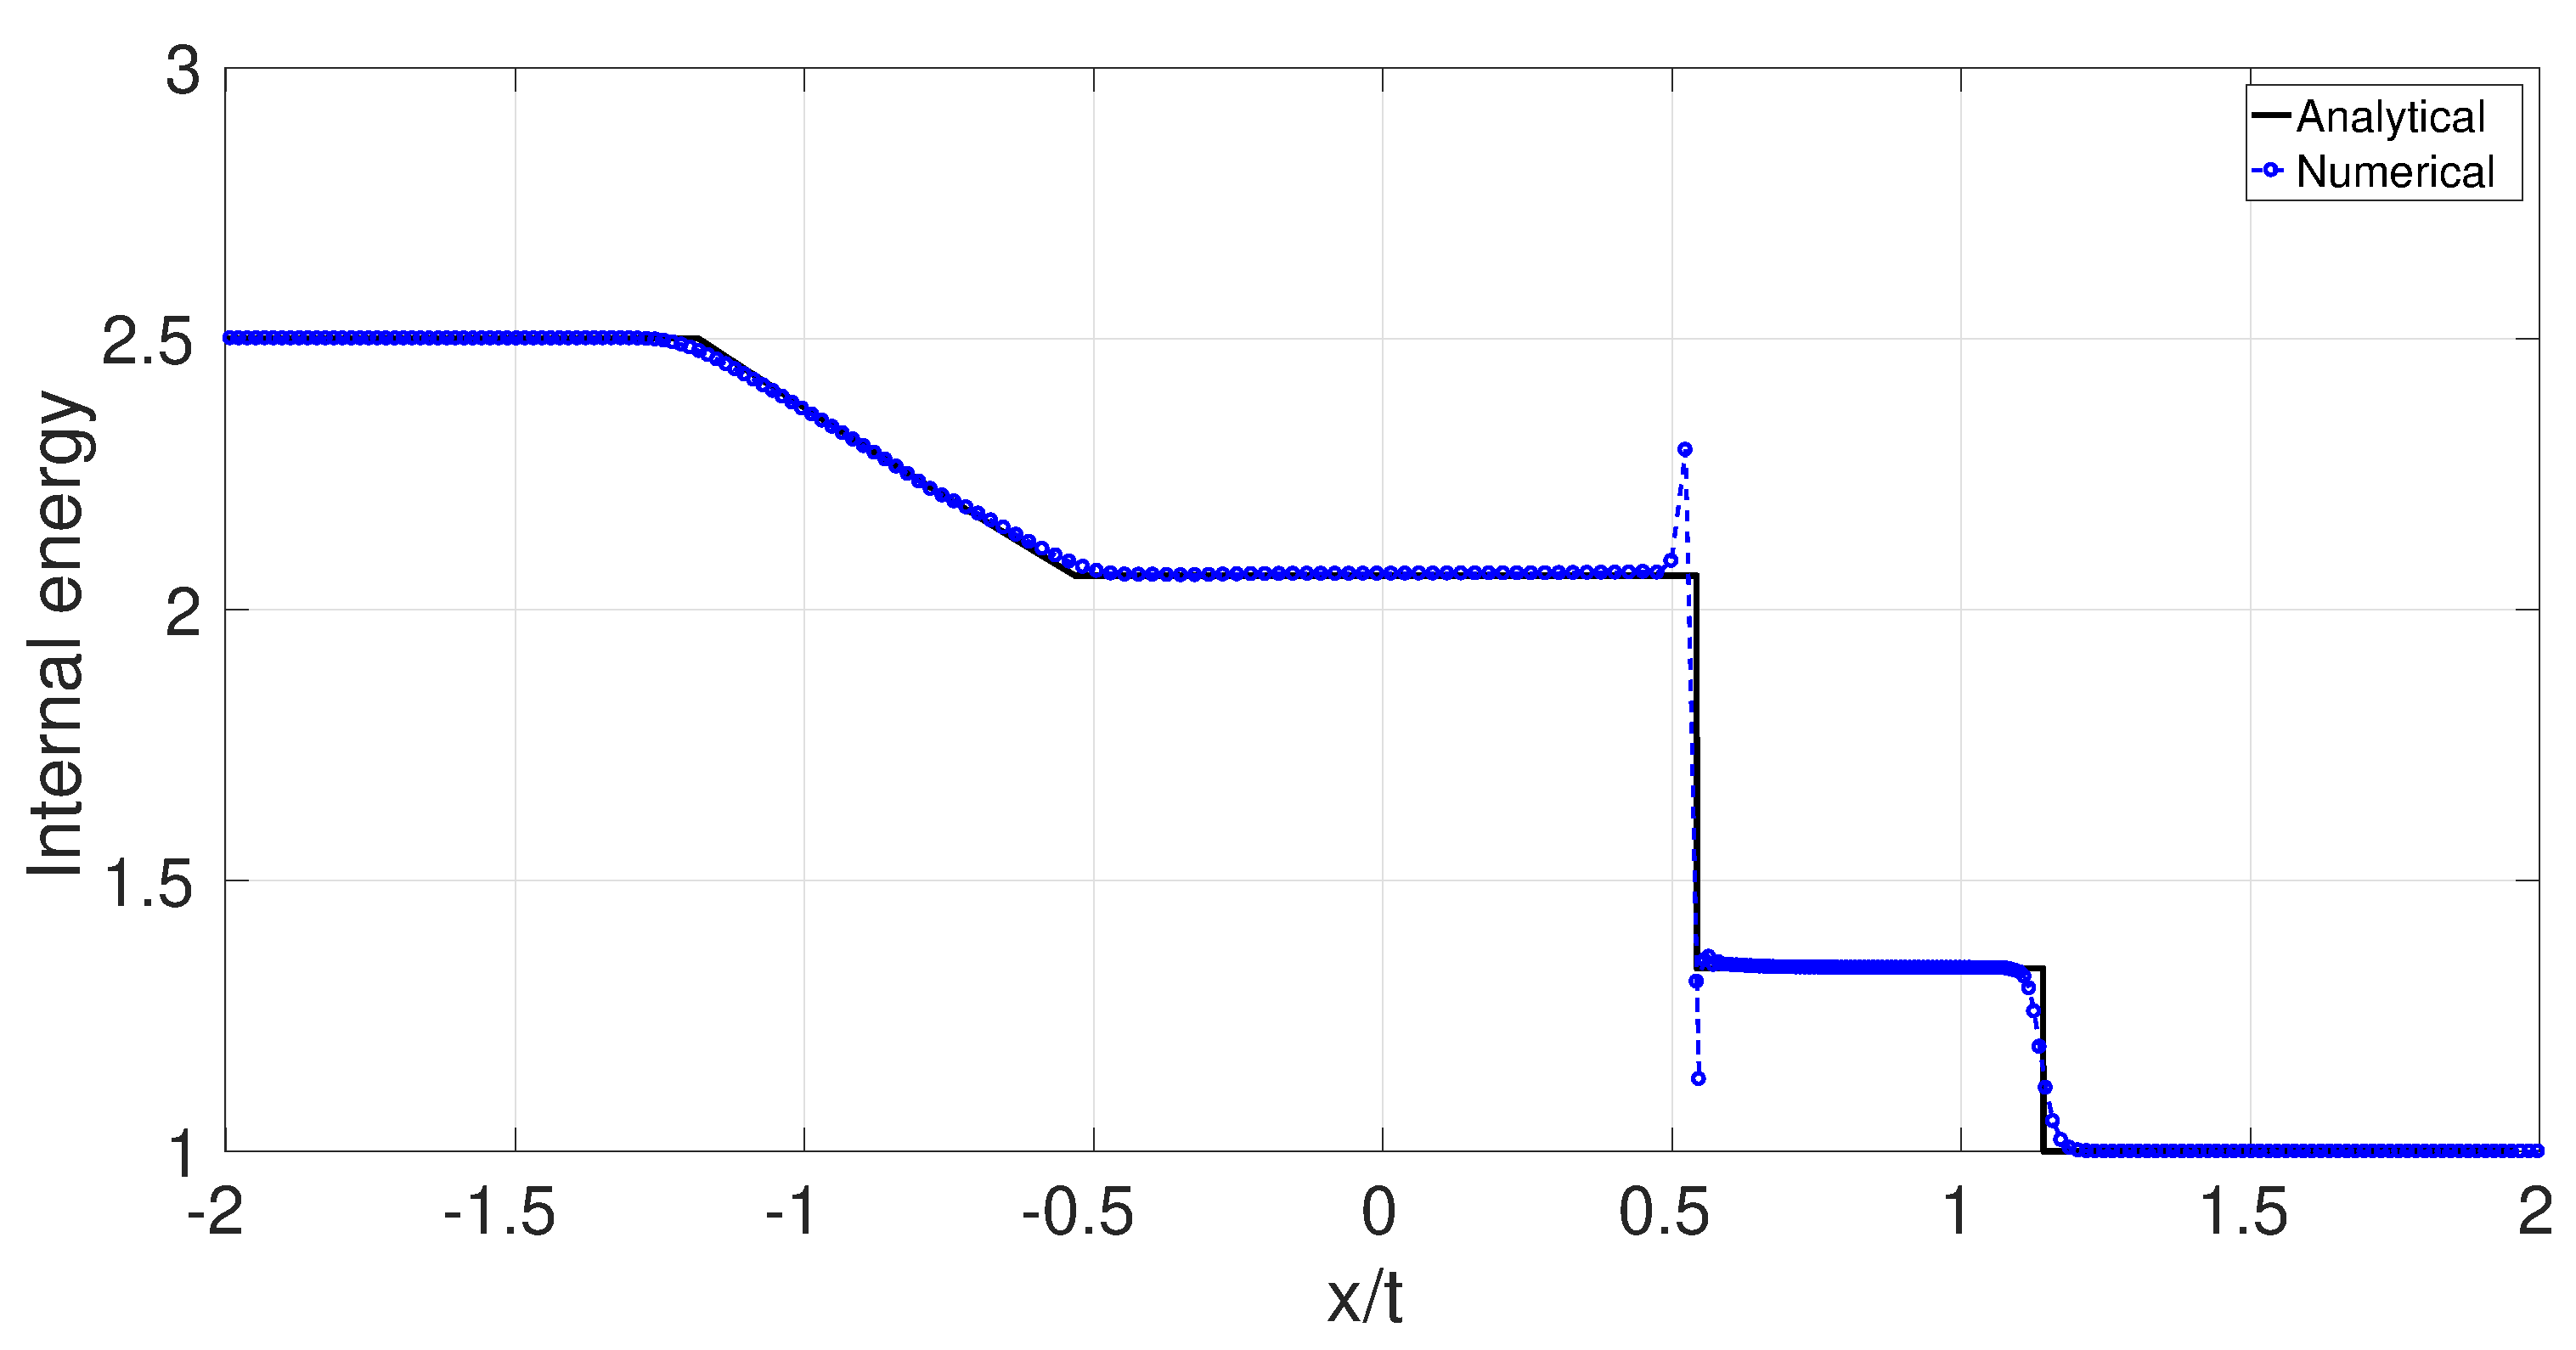
\includegraphics[width=0.99 \textwidth]{./GSPH-Sod-verification-e}
    \end{minipage}%
    \begin{minipage}{.325 \textwidth}
        \centering
        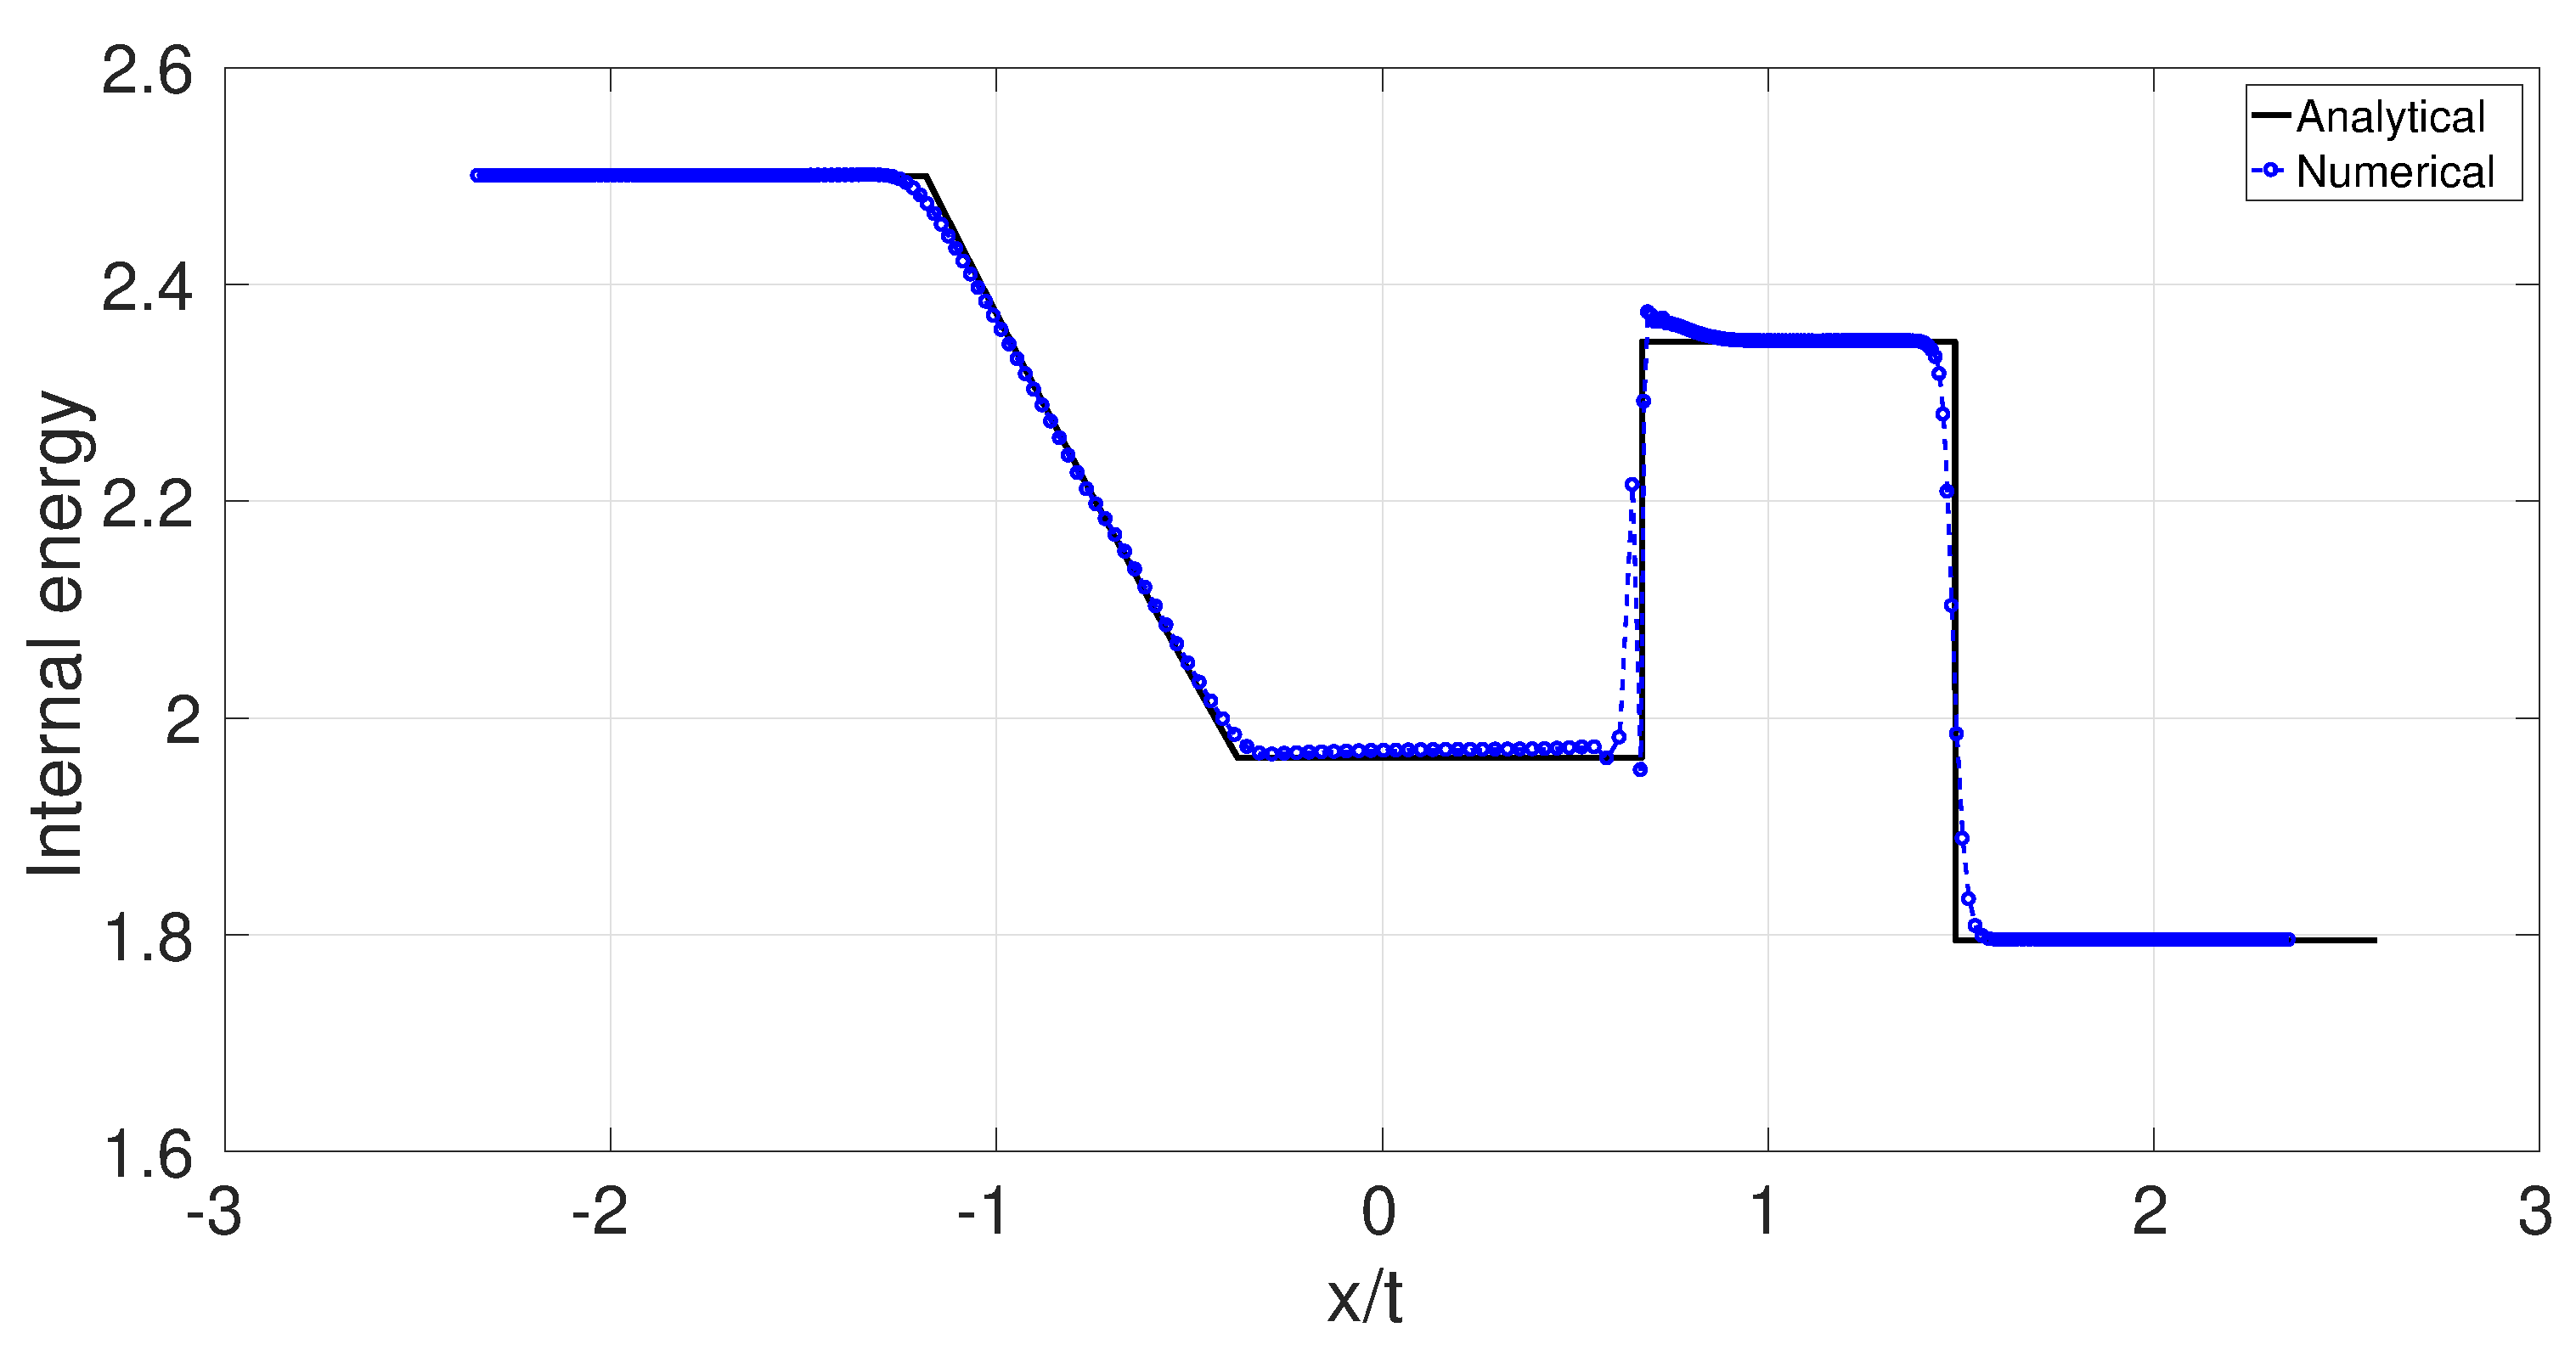
\includegraphics[width=0.99 \textwidth]{./Sod-verification-e}
    \end{minipage}%
    \begin{minipage}{.325 \textwidth}
        \centering
        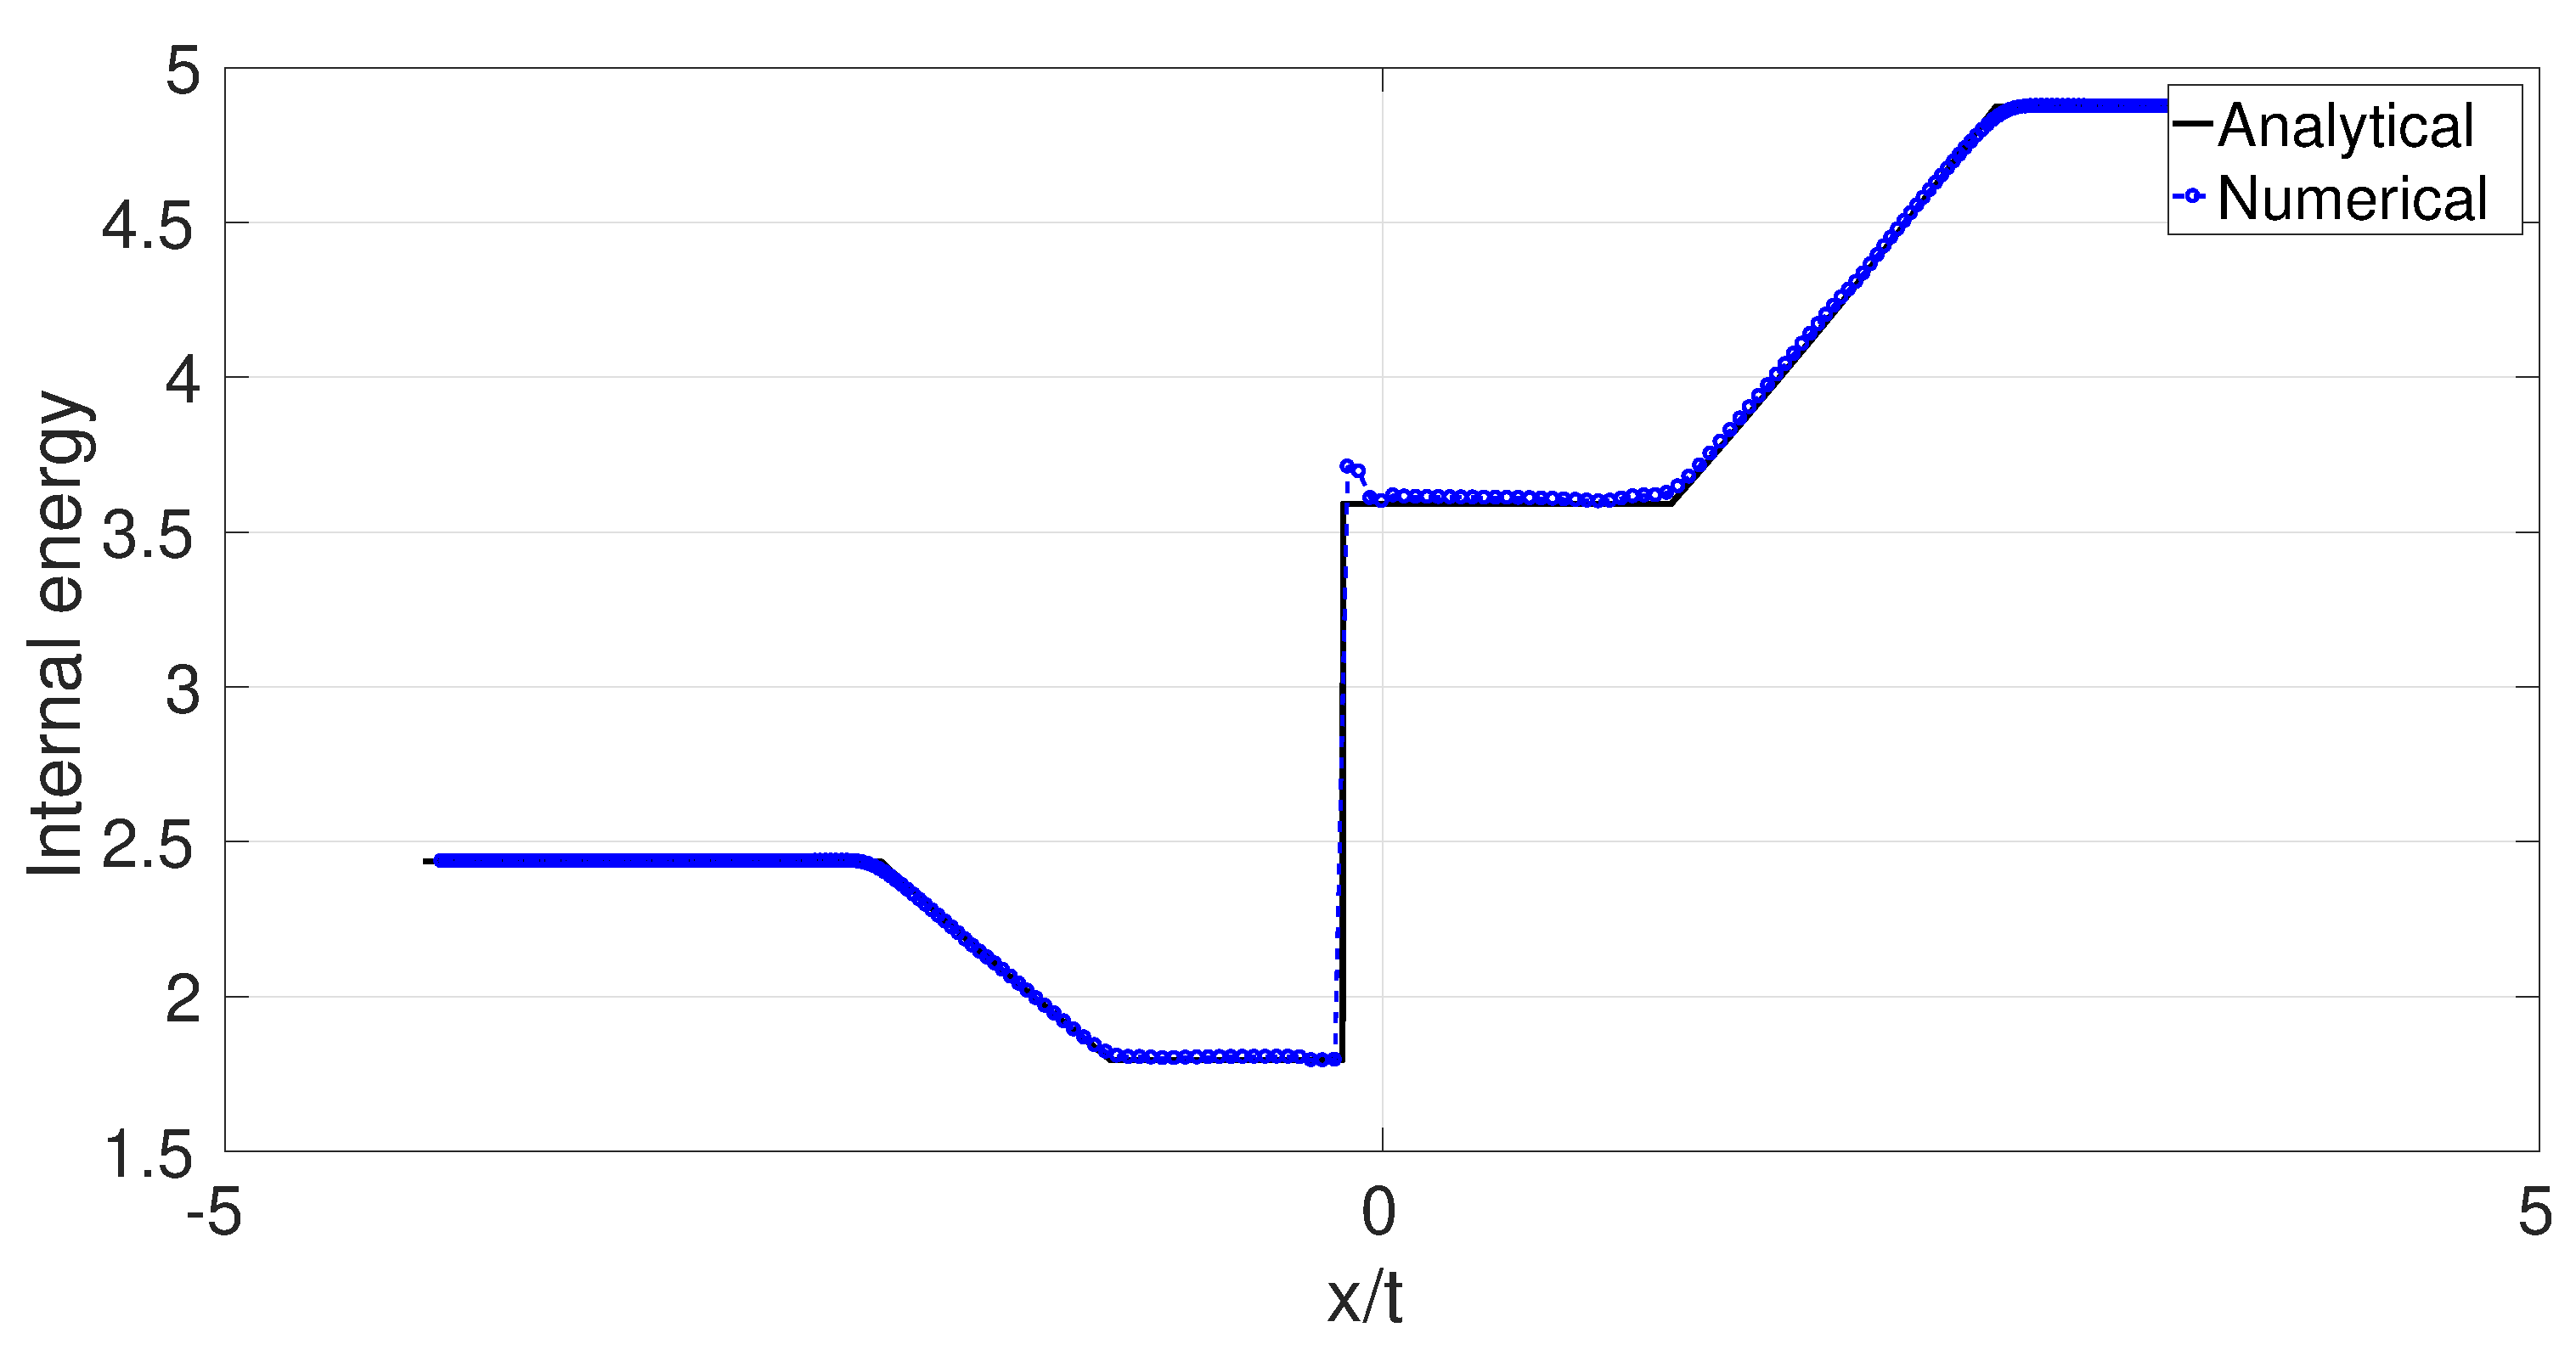
\includegraphics[width=0.99 \textwidth]{./d-exp-verification-e}
    \end{minipage}%   
    \caption{Comparison of specific internal energy of simulation results agaist analytical results for shock tube tests. The plots from left to right are corresponding to test 1, test 2 and test 3 respectively.}
    \label{fig:1D-shock-tests-verification}
\end{figure}

\subsection{Simulation of JPUE}
JPUE can be considered as a simplified volcanic plume. While the effect of stratified atmosphere and the effect of expansion due to high temperature in volcanic plume are not represented, JPUE reproduces the entrainment due to turbulent mixing which is one of the key elements in volcanic plume development. There exist consistently good experimental data \citep { list1982turbulent,dimotakis1983structure, papanicolaou1988investigations, ezzamel2015dynamical} that describe the JPUE flow field giving an insight into details of JPUE, such as transverse velocity and concentration profile. In this section, we verify that our code and the $SPH-\varepsilon$ turbulence model is able to reproduce feature of turbulent entrainment by a JPUE simulation.

As many of these experiments were conducted with liquid, we replace the original equation of state (Eq. (\ref{eq:EOS})) with a weakly compressible Tait equation of state \citep {becker2007weakly} (see Eq. (\ref{eq:EOS-Tait})) to avoid solving the Poisson equation.
\begin{equation}
p=B\left[\left(\dfrac{\rho}{\rho_0}\right)^{\gamma}-1\right]
\label{eq:EOS-Tait}
\end{equation}
with $\gamma=7$ and $B$ is evaluated by:
\begin{equation}
B=\dfrac{\rho_0 c^2}{\gamma}
\end{equation}
where $c$ is the speed of sound in the liquid. The energy equation is actually decoupled from the momentum conservation equation and the mass conservation equation by using this EOS. In addition, the "atmosphere" is assumed to be uniform and gravity is set to be zero. We set the temperature and density of ejected material the same as surrounding ambient. This further simplifies the scenario for the convenience of studying turbulent mixing. 

One overall feature of JPUE is "self-similarity" which means that the evolution of the JPUE is determined solely by the local scale of length and velocity, which theoretically account for the fact that the rate of entrainment at the edge of JPUE is proportional to a characteristic velocity at each height. As a results, physical and numerical experiments do not necessary to have exactly the same setups and are compared on a non-dimensional basis.

\begin{table}[htp]
	\begin{centering}
      \caption{List of eruption condition for the test cases}		
	  \begin{tabular}{lrrr}
	    \hline
	    Parameters & Units  & JPUE & Plume \\
	    \hline
	    Vent velocity          & $m\cdot s^{-1}$  & 500               & 275 \\
	    Vent gas mass fraction &                  & 1.0               & 0.05 \\
	    Vent Temperature       & $K$              & 273               & 1053 \\
	    Vent height            & $m$              & 0                 & 1500 \\
	    Mass discharge rate    & $kg\cdot s^{-1}$ & $5.47 \times 10^7$ & $1.5 \times 10^9$\\
	    \hline
	  \end{tabular}
	  \label{tab:input_parameters}
	\end{centering}
\end{table}

\begin{figure}[!htb]
    \centering
    \begin{minipage}{.425\textwidth}
        \centering
        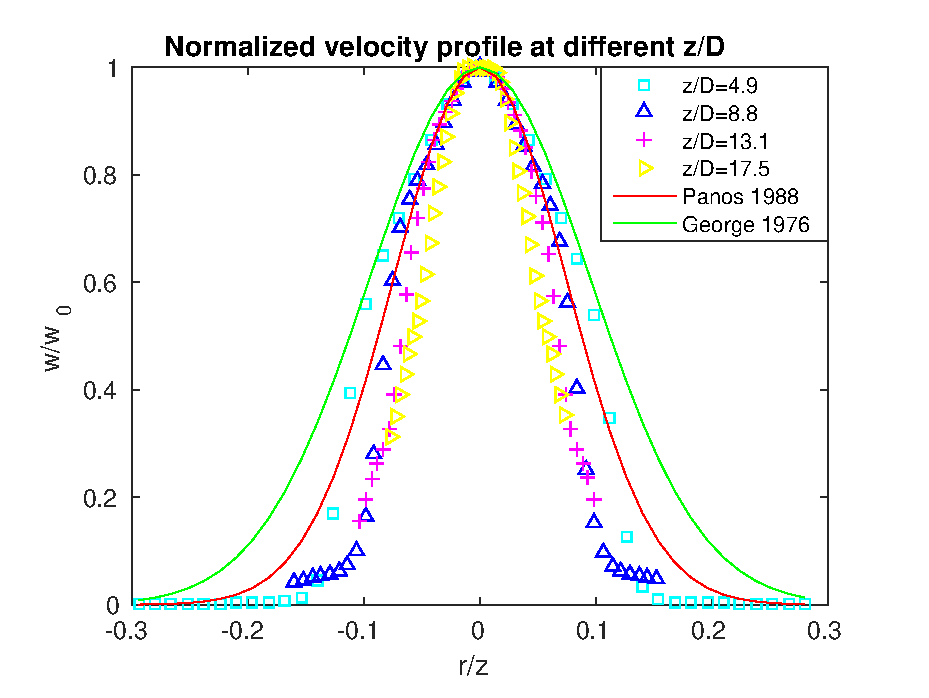
\includegraphics[width=8cm]{vel_cross}
    \end{minipage}%
    \begin{minipage}{.425 \textwidth}
        \centering
        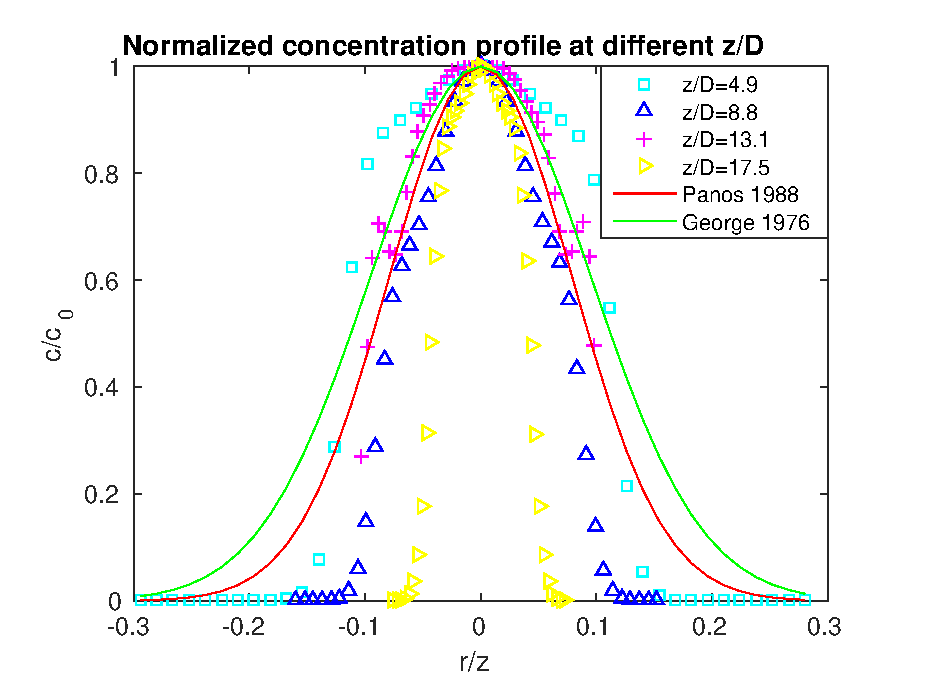
\includegraphics[width=8cm]{conc_cross}]
    \end{minipage}%  
    \caption{Dimensionless concentration and velocity distribution across the cross-section.}
    \label{fig:JPUE_cross-section}
\end{figure}

\begin{figure}[!htb]
    \centering
    \begin{minipage}{.425\textwidth}
        \centering
        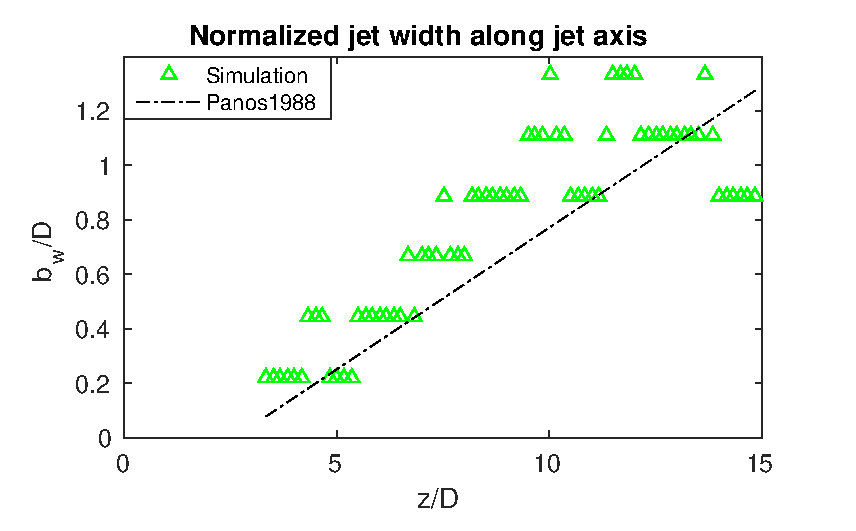
\includegraphics[width=8cm]{velo_along_axis}
    \end{minipage}%
    \begin{minipage}{.425 \textwidth}
        \centering
        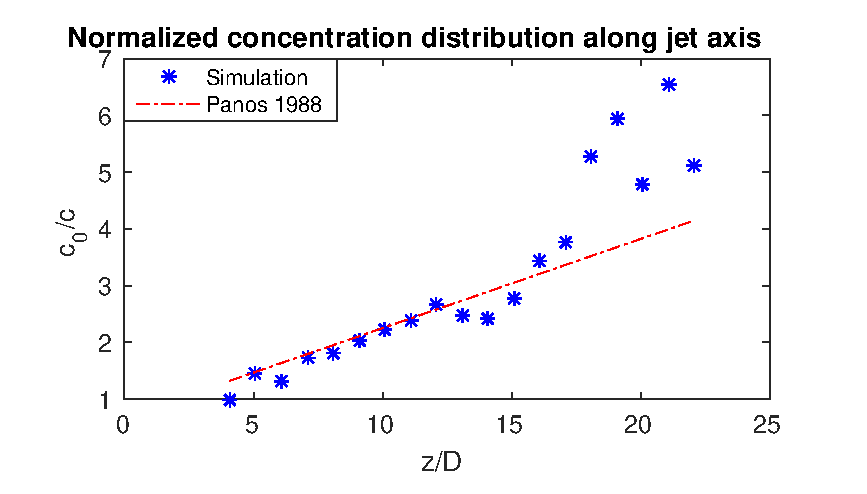
\includegraphics[width=8cm]{conc_along_axis}
    \end{minipage}%  
    \caption{The left plot is normalized jet width (which determined based on velocity) along the centerline. The right plot shows normalized concentration along the centerline.}
    \label{fig:JPUE_along-axis}
\end{figure}
%
%\begin{figure}
%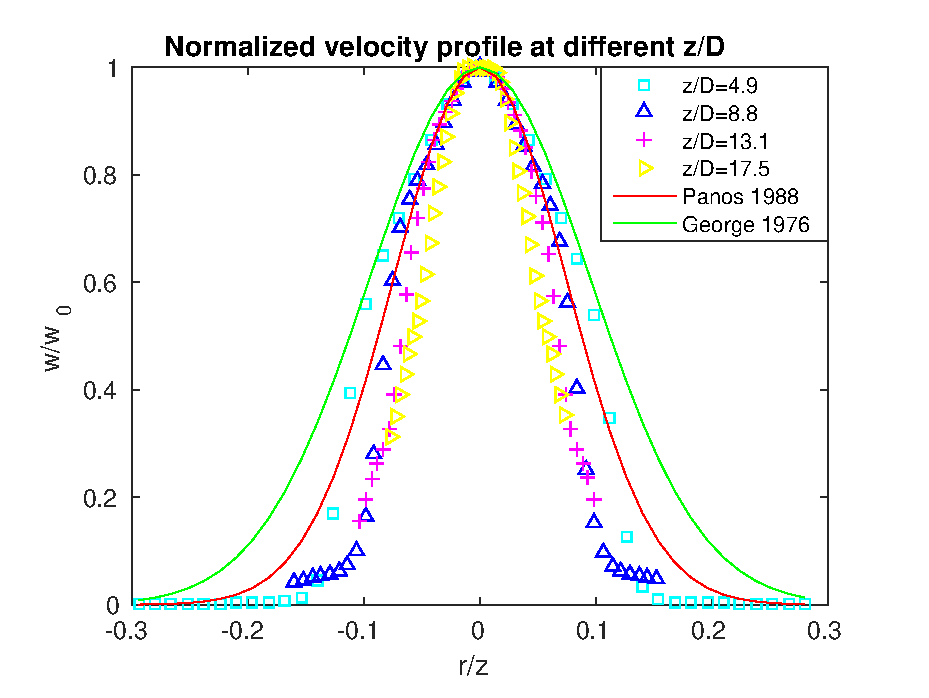
\includegraphics[width=8cm]{vel_cross}
%\caption{Dimensionless velocity distribution across the cross-section.}
%\label{fig:JPUE_cross-section_vel}
%\end{figure}
%
%\begin{figure}
%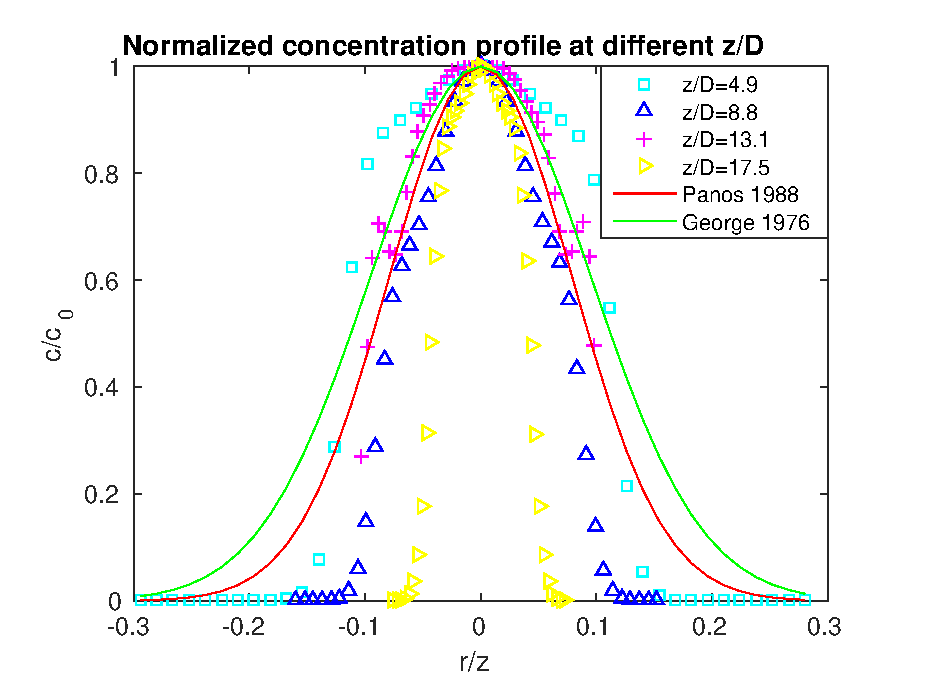
\includegraphics[width=8cm]{conc_cross}
%\caption{Dimensionless concentration distribution across the cross-section.}
%\label{fig:JPUE_cross-section_conc}
%\end{figure}

%\begin{figure}
%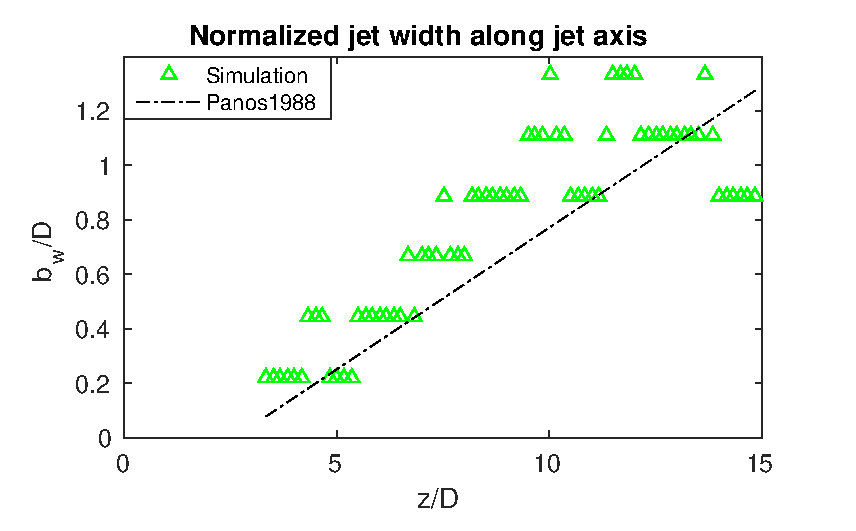
\includegraphics[width=8cm]{velo_along_axis}
%\caption{Dimensionless velocity and concentration distribution along centraline.}
%\label{fig:JPUE_along-axis_vel}
%\end{figure}
%\begin{figure}
%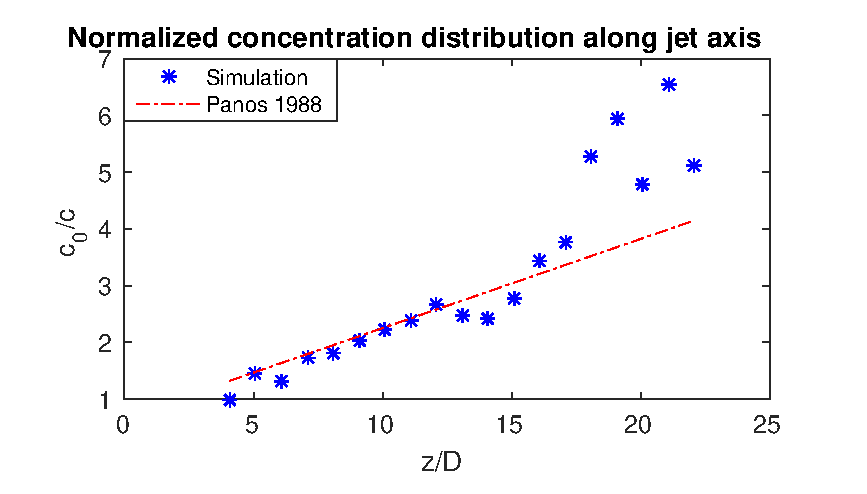
\includegraphics[width=8cm]{conc_along_axis}
%\caption{Dimensionless concetration distribution along centraline.}
%\label{fig:JPUE_along-axis_conc}
%\end{figure}

A three dimensional axisymmetric JPUE which ejects from a round vent is simulated with eruption parameters listed in Table \ref{tab:input_parameters}. Material properties of water are used as material properties for both phases. The results are compared with experiments \citep {george1977turbulence, papanicolaou1988investigations} for verification purposes. Experimental data of concentration and velocity distribution across the cross-section were fit into a Gaussian profile (See Eq. (\ref{eq:JPUE-experiment-fit-corss})) by \citet{papanicolaou1988investigations} and  \citet{ george1977turbulence} even though the actual profile are slightly different from the Gaussian profile.

\begin{equation}
\dfrac{\varphi}{\varphi_c}=exp \left[-coef\left( \left(\dfrac{r}{z}\right)^2\right)\right]
\label{eq:JPUE-experiment-fit-corss}
\end{equation}

where $\varphi$ is either velocity or concentration, the subscript $c$ represents the centreline. $r$ is the distance from the centreline on any cross-section. $z$ is the axial distance from the origin of the jet transverse section under consideration. 
The coefficient $coef$ for concentration is 80 and 50 respectively according to \citet{george1977turbulence} and \citet{papanicolaou1988investigations}.
$coef$ for velocity is 90 and 55 respectively according to \citet{george1977turbulence} and \citet{papanicolaou1988investigations}. 

\citet{papanicolaou1988investigations} also fit concentration distribution and jet width based on velocity along centerline into a straight line (See Eq. (\ref{eq:JPUE-experiment-fit-along-axis})).. 

\begin{equation}
\dfrac{\varphi_0}{\varphi_c}=slope \left(\dfrac{z}{D} + intercept \right)
\label{eq:JPUE-experiment-fit-along-axis}
\end{equation}

where subscript $0$ represents the cross-sectionally averaged exit value, $D$ is the diameter of vent. 
$slope$ for jet width based on velocity is 0.104 and for concentration is 0.157. 
$intercept$ for jet width based on velocity is 2.58 while that for the concentration is 4.35.

Although both velocity and concentration are found to be well matched with experimental results, a small disparity in both velocity and concentration are observed near the boundary of the jet. Which is possibly caused by overestimating of the drag effect by standard SPH \citep {ritchie2001multiphase}. \citet {ritchie2001multiphase} also proposed an alternative way for density update which releived the overestimating of the drag effect. However, how well does his method conserve mass is not clear. There are several other factors that might also attribute to such disparity. Reynolds number is not reported in many experiments assuming a high enough Reynolds number. In addition, some details of the experiments, such as exit velocity profile and viscosity of the experimental liquid, are not reported. These factors prevent us from numerically reproducing these experiments in an exact way as they were conducted. However, the features of JPUE are correctly reproduced with our code.

We also investigated the mixing due to turbulence in JPUE simulation by checking the mixture of the two phases. It is shown in Fig. \ref{fig:Turb_mixing} that the ejected material and ambient fluids are mixed through eddies at the outer shear region. And the inner dense core dispersed gradually due to erosion of the outer shear region. Hence, our confidence in the numerical correctness of our code is greatly reinforced.
%What need to be noticed is that the mass of particle of phase 1 (blue) is 8 time of that of phase 2 (red). It is a trade off between resolution and computational expense to give particle of two phases different particles mass. Both advanced SPH techniques like adaptive particles size and better data management and access strategies need to be exploited to address this issue.

\begin{figure}
\includegraphics[width=8cm]{JPUE_entrainment.png}
\caption{The left figure shows particle distribution. Particles of phase 1 (blue) are gradually entrained and mixed with erupted particles (red) as jet flows down stream. The right figure shows the mass fraction of erupted material at the moment corresponding to the left figure.}
%What need to be noticed is that the mass of particle of phase 1 (blue) is 8 time of that of phase 2 (red). It is a trade off between resolution and computational expense to give particle of two phases different particles mass.
\label{fig:Turb_mixing}
\end{figure}

\subsection{Simulation of a volcanic plume}
The development of a volcanic plume is more complicated than JPUE in several aspects. Besides turbulent entrainment of ambient fluids, development of volcanic plume also involves heating up of entrained air and expanding in a stratified atmosphere. A strong eruption column without wind is tested in this section for the purpose of further verification and validation.
Both global variable and local variables are compared with existing models.

\subsubsection{Input parameters}
Eruption parameters, material properties and atmosphere are chosen to be the same as the strong plume no wind case in a comparison study on eruptive column models by \citet {costa2016results}. Eruption conditions are listed in Table \ref{tab:input_parameters}. As our model does not distinguish solid particles of different sizes, only mass fraction of solids of all size is used in simulation even though two size classes were provided by \citet {costa2016results}. The density of erupted material at the vent and radius of the vent can be computed from the given parameters. The eruption pressure is assumed to be as the same as pressure of ambient at the vent and hence is not given in the table. The vertical profiles of atmospheric properties were obtained based on the reanalysis data from ECMWF (European Centre for Medium-Range Weather Forecasts) for the period corresponding to the climactic phase of the Pinatubo eruption (Philippines, 15 June 1991). These conditions are more typical of a tropical atmosphere (see Fig. 1B in \citep{costa2016results}). 
%Wind speed is not used in our current model even though it is given (by one component speed from west to east and another component speed from south to north). 
Vertical distribution of temperature, pressure and density is used to establish stratified atmosphere. Wind velocity and specific humidity are not used in our simulation even though they were also provided by \citet{costa2016results} (see Fig. 1B). Material properties, shown in Table \ref{tab:material_properties}, are selected based on properties of Pinatubo and Shinmoe-dake eruption. Other material properties not given in the table can be inferred from these given parameters based on their relationships.

\begin{table}[htp]
	\begin{centering}
      \caption{List of material properties}		
	  \begin{tabular}{lrrr}
	    \hline
	    Parameters & Units  & Value \\
	    \hline
	    	Specific heat of gas at constant volume     & $J \cdot kg^{-1}\cdot K^{-1}$& 717     \\
	    Specific heat of air at constant volume     & $J \cdot kg^{-1}\cdot K^{-1}$& 1340    \\
	    	Specific heat of solid                      & $J \cdot kg^{-1}\cdot K^{-1}$& 1100    \\
	    	Specific heat of gas at constant pressure   & $J \cdot kg^{-1}\cdot K^{-1}$& 1000    \\
	    	Specific heat of air at constant pressure   & $J \cdot kg^{-1}\cdot K^{-1}$& 1810    \\
	    	Density of air at vent height               & $kg \cdot m^{-3}$       & 1.104   \\
	    Pressure at vent height                        & $Pa$              & 84363.4 \\
	    \hline
	  \end{tabular}
	  \label{tab:material_properties}
	\end{centering}
\end{table}

Figure \ref{fig:pinatubo-simulation-results-vis} shows the mass fraction of simulated volcanic plume at 500s after eruption, at which time the plume starts spreading radially. A contour plot of the mass fraction on the vertical cross-section (x-z plane) were also provided. The zoomed view of the quivier plot shows detailed entrainment of air at the margin of the plume.

\begin{figure}[!htb]
    \centering
    \begin{minipage}{.45\textwidth}
        \centering
        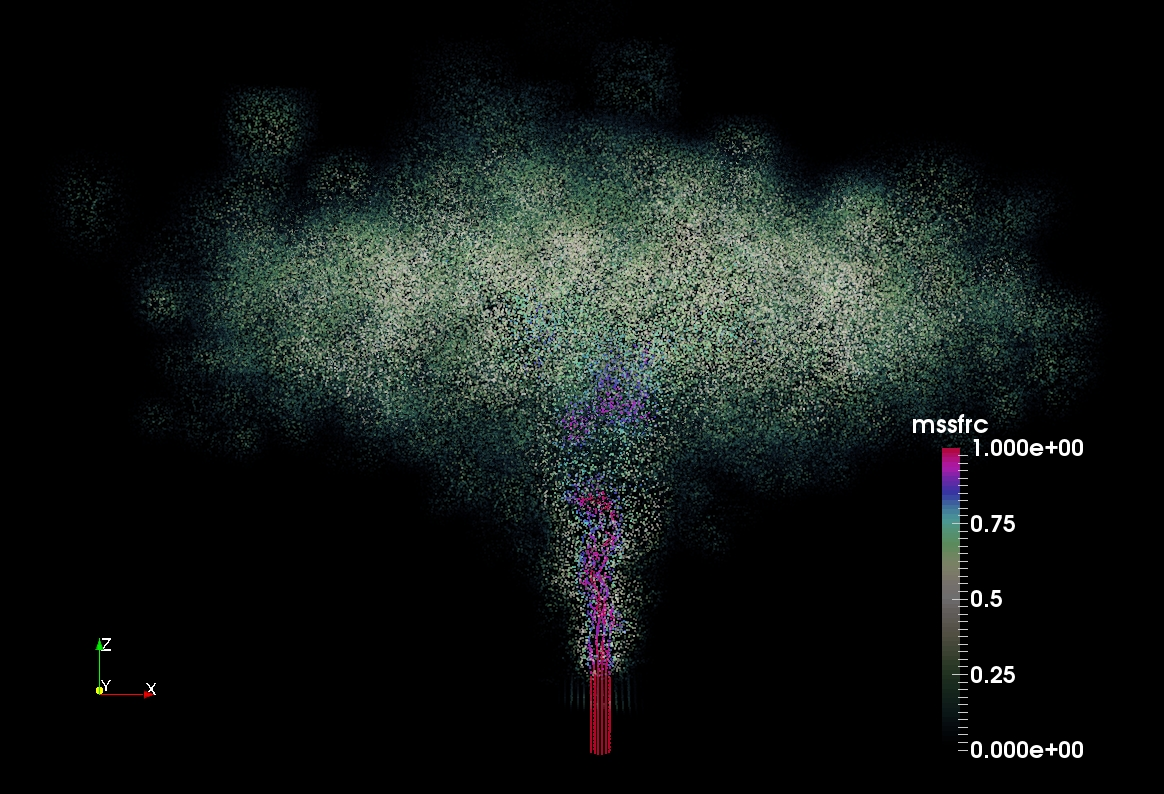
\includegraphics[width=0.99 \textwidth]{./mssfrc-Diverging}
    \end{minipage}%
    \begin{minipage}{.45 \textwidth}
        \centering
        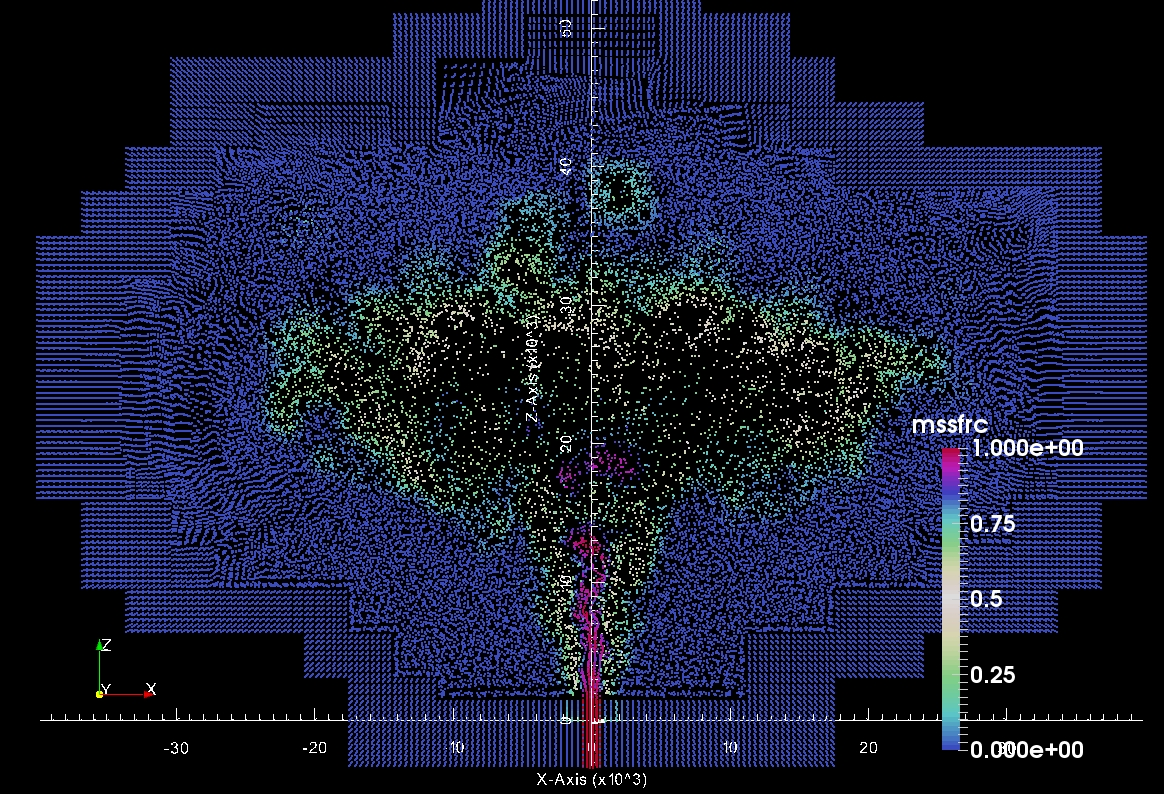
\includegraphics[width=0.99 \textwidth]{./mssfrc-Diverging-cut}
    \end{minipage}%
    \\
    \begin{minipage}{.45 \textwidth}
        \centering
        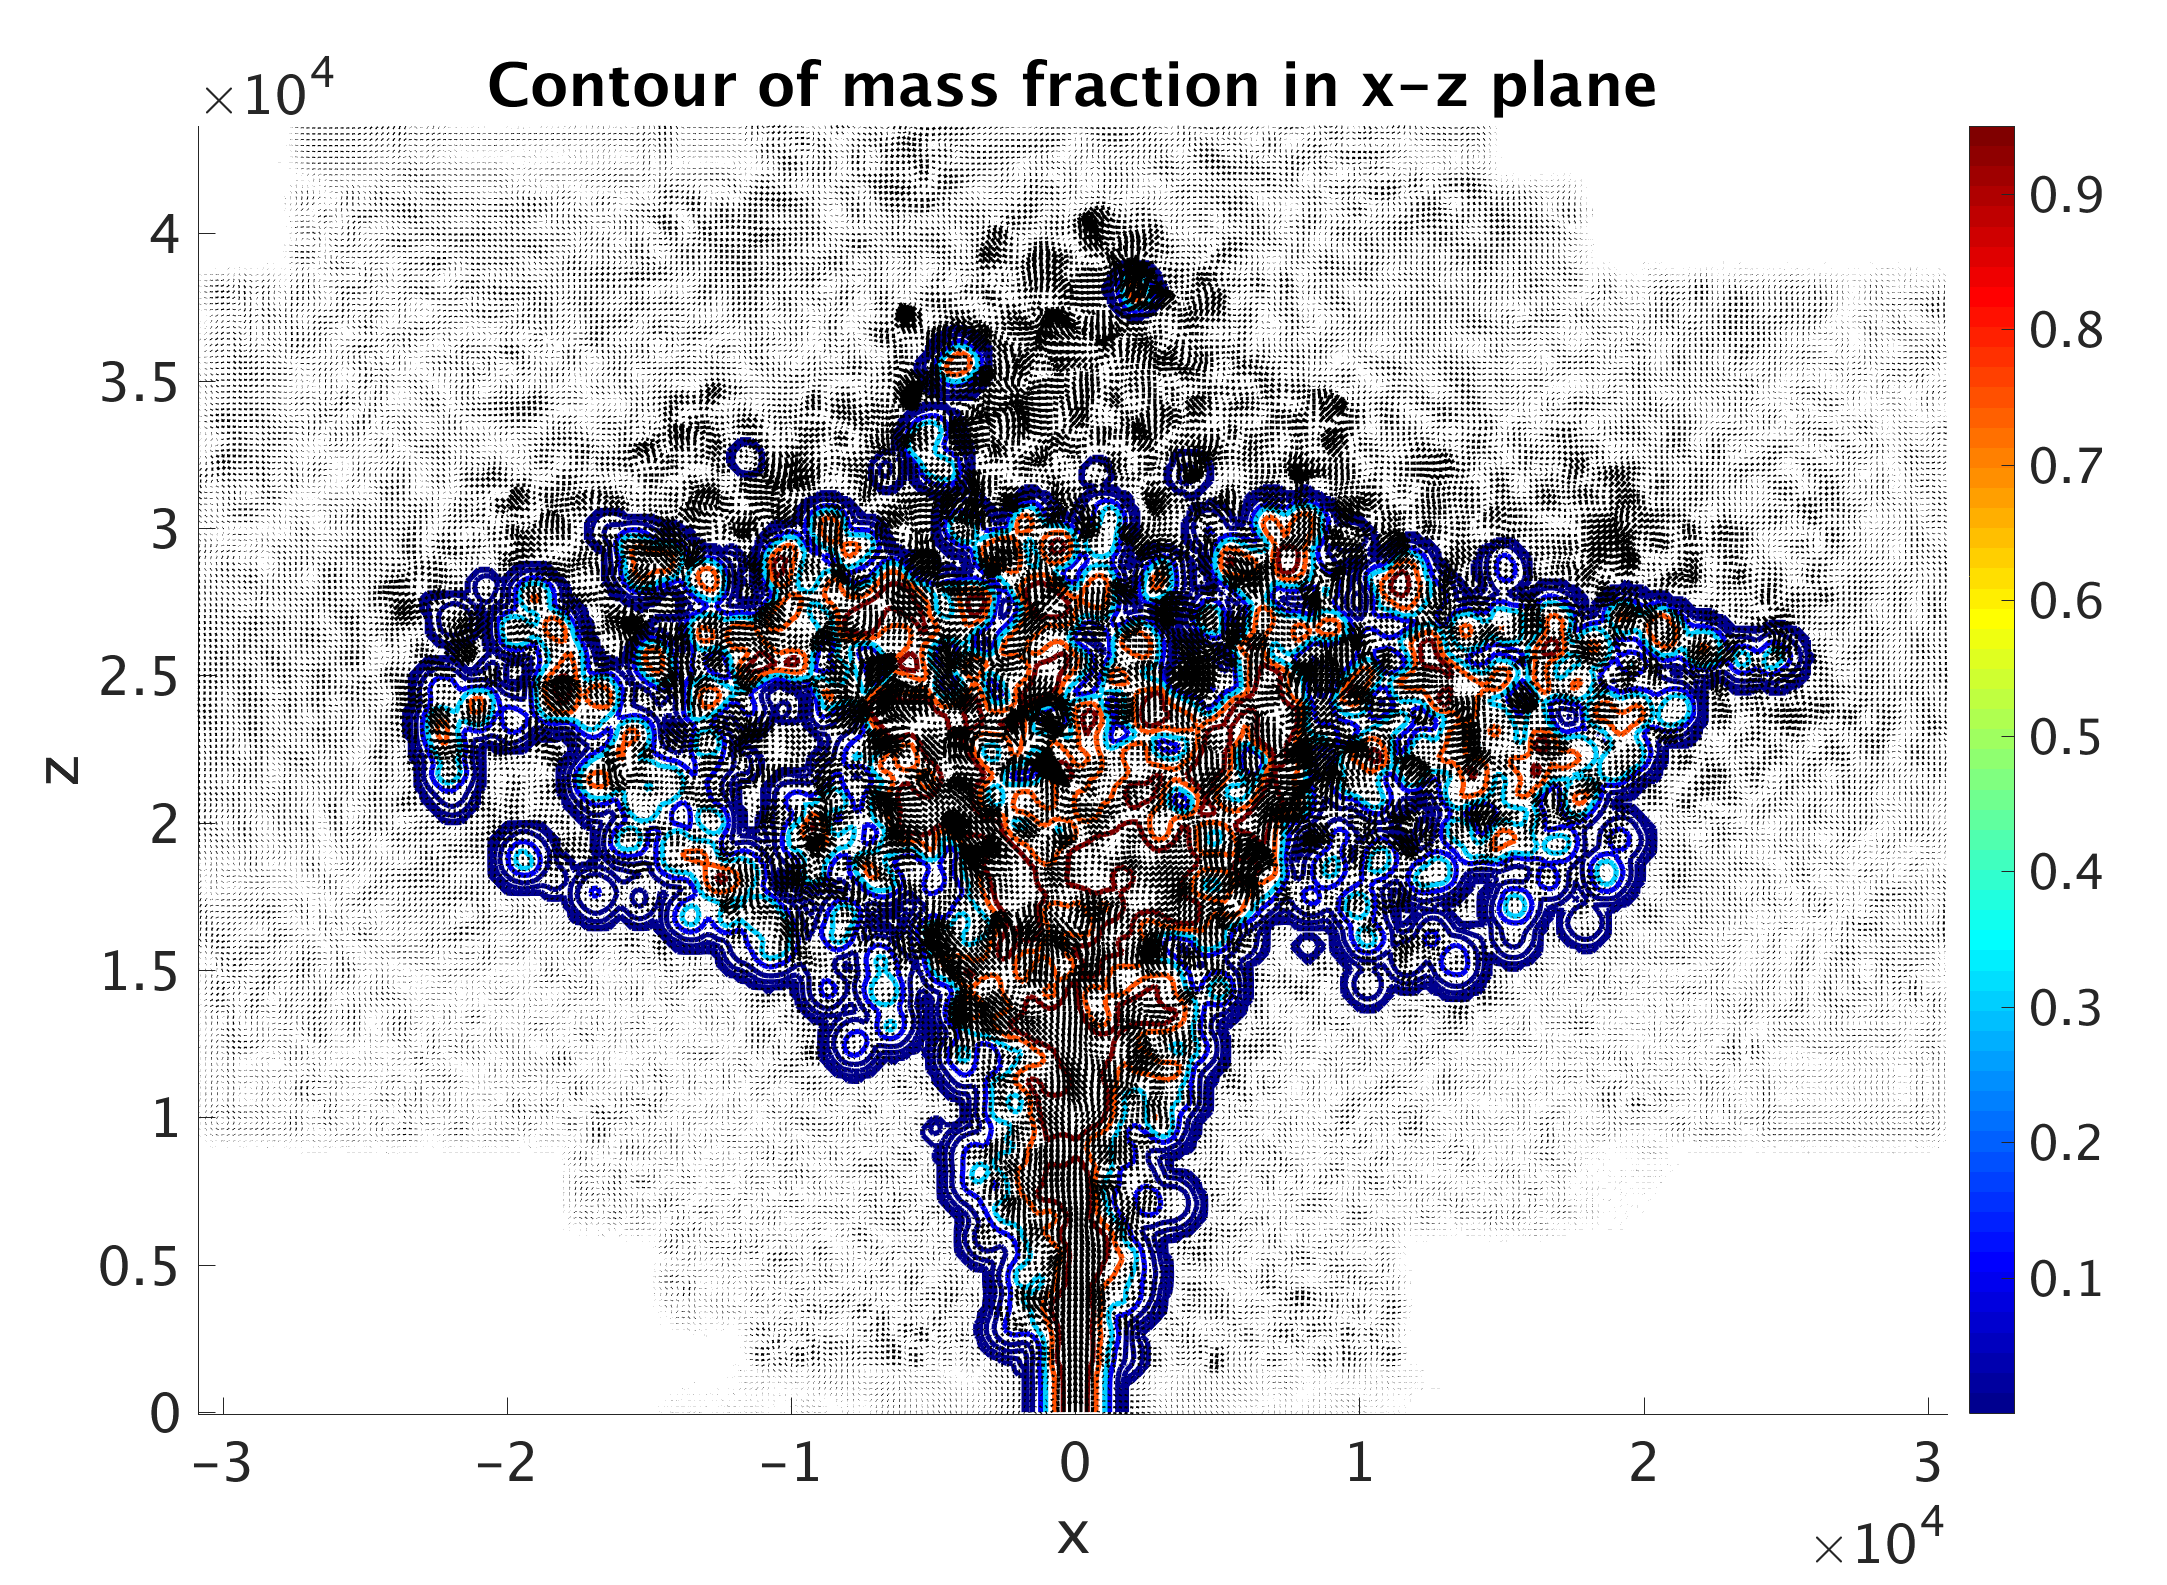
\includegraphics[width=0.99 \textwidth]{./gmd-mssfrc-xz}
    \end{minipage}% 
    \begin{minipage}{.45 \textwidth}
        \centering
        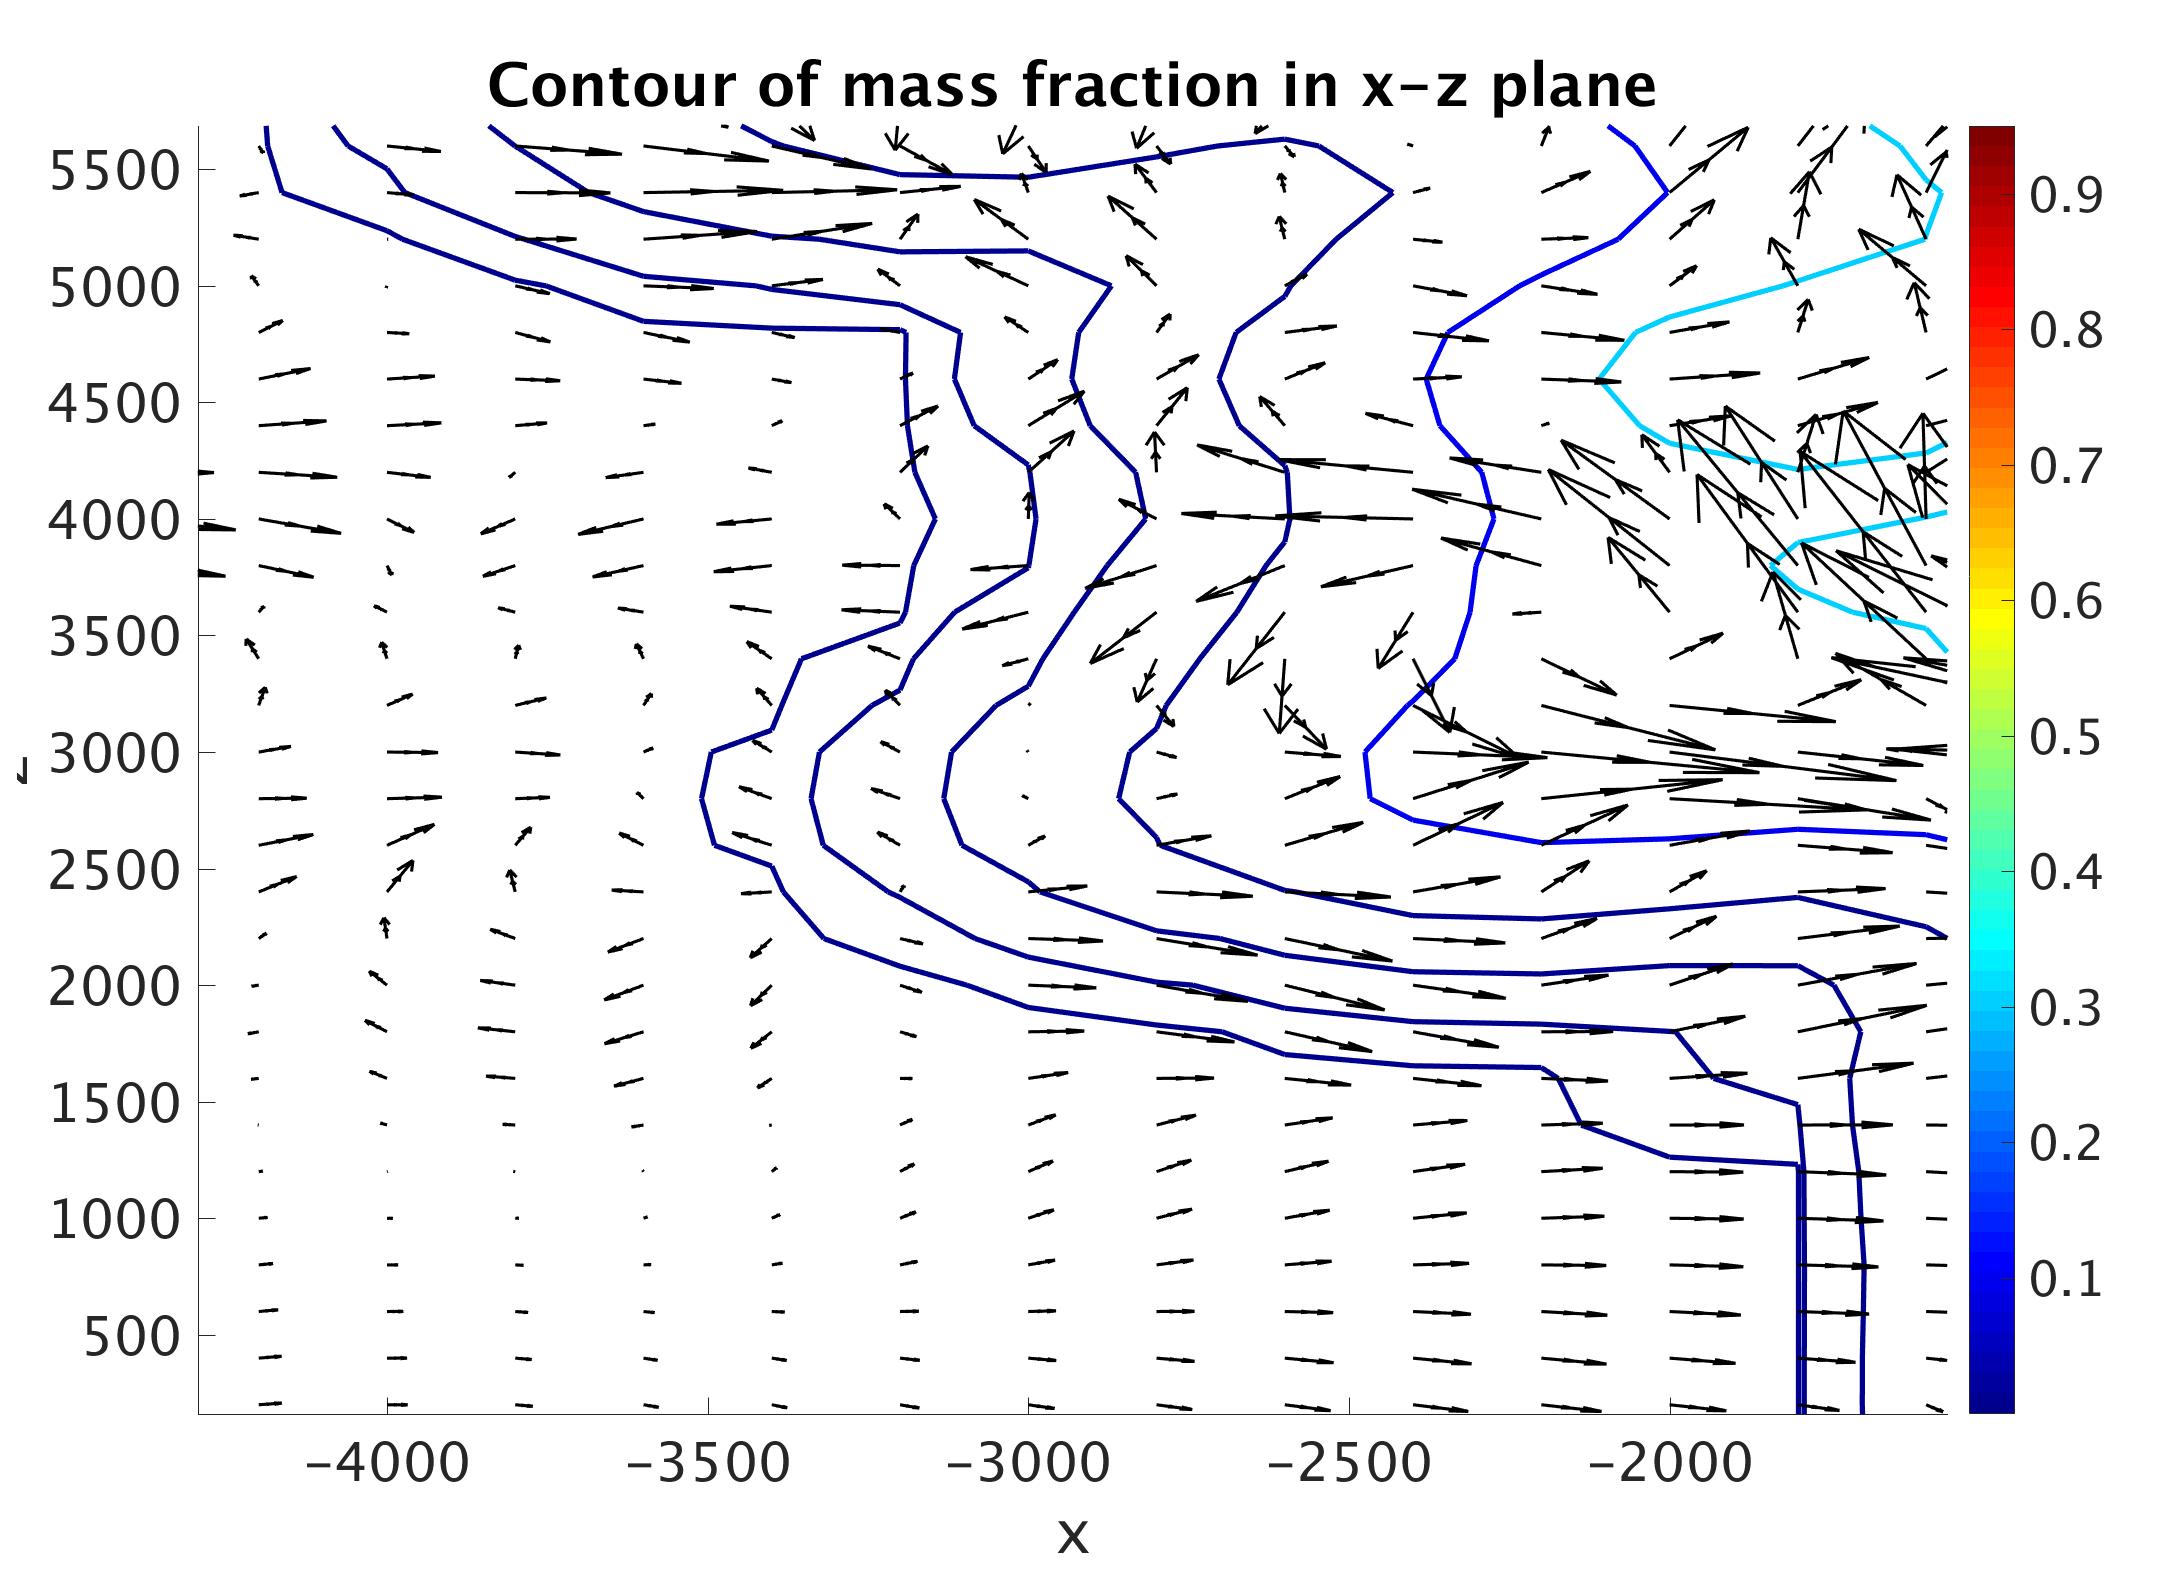
\includegraphics[width=0.99 \textwidth]{./gmd-mssfrc-xz-zoomed}
    \end{minipage}%  
    \caption{Mass fraction for $t=500s$ after eruption. Figures on the first row are visualization of SPH simulation results. The figure on the up right corner is visualization of a slice of the computational, whose thickness is around $10000m$. The lowest portion of the plume represents erupted material in eruption vent (the underground portition). Figures at the second row show contour of mass fraction and velocity quiver on x-z plane. These figures are plotted utilizing post-processed data (see Appendix \ref{app:project-SPH-grid}). The contour level in the plot are $0.00001, 0.0001, 0.001, 0.1, 0.3, 0.75, 0.95$. The figure on the lower right corner is a zoomed view of velocity quivier showing plume expansion and entrainment of air.}
    \label{fig:pinatubo-simulation-results-vis}
\end{figure}

\subsubsection{Global and local variables}
One of the key global quantities of great interest is the altitude to which the plume rises. The top height predicted by our model is around 40 km which agrees with other plume models. For example, the height predicted by PDAC is 42500 m, by SK-3D is 39920 m, by ATHAM is 33392 m, by AHSEE is 36700 m. As for local variables, the profiles of integrated temperature, density, mass fraction of entrained air, gas mass fraction, mass fraction of solid and the radius of the plume as a function of height are compared with existing 3D models in Fig. \ref{fig:strong_local_temp} $\sim$ \ref{fig:strong_local_radius}. To get rid of significant fluctuations in time and space we conducted a time averaging and spatial integration of the dynamic 3D flow fields by following \citet {cerminara2016large}.

As particles distribute irregularly in the space in SPH simulation results. We need to project simulation results (on irregular particles) onto a pre-defined grid before doing time average and spatial integration. See appendix A for more details of post processing.

The profiles of local variables match well with simulation results of existing 3D models in a general sense. The basic phenomena in volcanic plume development is correctly captured by our model.

\begin{figure}
\center
\includegraphics[width=7cm]{Temp}
\caption{Temperature as a function of height}
\label{fig:strong_local_temp}
\end{figure}

\begin{figure}
\includegraphics[width=15cm]{msfrac}
\caption{The mass fraction of entrained air, gas, and solid as a function of height.}
\label{fig:strong_plume_mass_fraction}
\end{figure}

As the height increases, the amount of entrained air also increases. Around the neutral height, where the umbrella expands, the entrainment of air shows a slight decrease due to lack of air surrounding the column at that height. The profile for gas, which account for both air and vapor, shows a very similar tendency as that of entrained air. Recall that vapor condensation is not considered in our model. In addition, we assume that erupted material behaves like a single phase fluid. So the mass fraction of gas is simply a function of entrained air (Eq. (\ref{eq:gas-frac-express})).
\begin{equation}
\xi_a + \xi_g = \xi_a + \left(1-\xi_a\right) \xi_{g0}
\label{eq:gas-frac-express}
\end{equation}
 
Among these 3D models, ATHAM takes vapor condensation into account and Eq. (\ref{eq:gas-frac-express}) does not hold for ATHAM. However, the profile of entrained air and profile of gas predicted by ATHAM are still very close to each other which implies that ignoring of water phase change is a valid assumption for eruptions similar to this test case (strong plume with erupted water fraction in erupted material less than 5\%). This observation can be explained by the fact that air occupies a larger portion of the gas and ignoring of phase change of vapor (which is only a small portion of gas) causes slight influence on plume development. As for mass fraction of solid, similarly, Eq. (\ref{eq:solid-frac-express1}) and Eq. (\ref{eq:solid-frac-express2}) hold for our model. 
\begin{equation}
\xi_s = \left(1 - \xi_a\right) \left(1- \xi_{g0}\right)
\label{eq:solid-frac-express1}
\end{equation}
\begin{equation}
\xi_s = 1 - \left(\xi_a + \xi_g\right)
\label{eq:solid-frac-express2}
\end{equation}

PDAC, which treats particles of two different sizes as two separate phases, predicted a similar mass fraction profile. That implies that assumption of dynamic equilibrium in our model is at least valid for eruptions similar to the test case.

With more cool air entrained into the plume and mixing with the hot erupted material, the temperature of the plume decreases as the height increases as shown in Fig. \ref{fig:strong_local_temp}. In the meanwhile, bulk density decrease due to entrainment and expansion (Fig. \ref{fig:strong_local_density}).
\begin{figure}
\center
\includegraphics[width=7cm]{density_strong}
\caption{Density of the strong plume without wind after reaching its top height}
\label{fig:strong_local_density}
\end{figure}
\begin{figure}
\center
\includegraphics[width=7cm]{radius_strong}
\caption{Radius of the strong plume without wind after reaching its top height.}
\label{fig:strong_local_radius}
\end{figure}
Our model adopts the same assumptions and governing equations as SK-3D. However, there is still an obvious disparity between the profiles of local variables of our model and SK-3D. One of the big differences between these two models is that we adopt a LANS type of turbulence model while SK-3D adopts a LES (large eddy simulation) turbulence model. This implies that choice of  turbulence model might play a critical role in plume simulation.

%\subsubsection{Evolution of plume} 
%
%\begin{figure}
%\center
%\includegraphics[width=15cm]{strong_elevation}
%\caption{This figure shows the dynamic evolution process of the Pinatubo with time. At the very beginning, it is driven by initial momentum and rises up quickly, mixing and entraining surround air. Around 100s, the jet stage finishes and it becomes a plume as there were enough air entrained. The plume keeps rising up until reaches the top height then starts spreading.}
%\label{fig:strong_evolution}
%\end{figure}
%
%\begin{figure}
%\includegraphics[width=10cm]{t50}
%\caption{Contour of mass fraction and velocity quiver at 50 seconds in plane x=0, the column keeps rising up and at the same time entraining air into the plume. The zoomed view (right figure) of the quiver plot clearly shows mechanism of air entrainment. The contour levels of mass fraction are 0.7, 0.5, 0.3, 0.1, $1\times 10 ^{-1}$, $1\times 10 ^{-2}$, $1\times 10 ^{-3}$, $1\times 10^{-4}$ and $1\times 10^{-5}$.}
%\label{fig:strong_plume_t50}
%\end{figure}
%
%Figure \ref{fig:strong_evolution} shows the overall evolution process of plume. Plume keeps rising up and entraining air into the plume until it reaches its top height(around t=300 seconds). Afterwards the mixtures of erupted material and air then fall back to neutral height and starts spreading radially. Detailed velocity quiver plot in Fig. \ref{fig:strong_plume_t50} shows entraining of air into the plume at the edge of column. The evolution of the plume further verifies our model.

\conclusions  \label{sec:conclusion}%% 
A new plume model was developed based on the SPH method. Extensions necessary for Lagrangian methodology and compressible flow were made in the formulation of the equations of motion and turbulence models. Advanced numerical techniques in SPH were exploited and tailored for this model. High performance computing was used to mitigate the tradeoff between accuracy (depends on comprehensiveness of the model, resolution, order of accuracy of numerical methods, scheme for time upgrading) and simulation time (depends on comprehensiveness of model, resolution, order of accuracy of numerical methods, scheme for time upgrading ... and computational techniques). The correctness of the code and model was verified and validated by a series of test simulations. Typical 1D shock tube problems were simulated and compared against analytical results showing good agreement. Dimensionless velocity and concentration distribution across the cross-section and along the jet axis match well with experimental results of JPUE. Top height and integrated local variables simulated by our model are consistent with simulation results of existing 3D plume models. Comparison between our results with those of SK-3D implies that turbulence model plays a significant role in plume modeling.

Currently existing 3D models focus on certain aspect of the volcanic plume (PDAC on pyroclastic flow, ATHAM on microphysics, and SK-3D on entrainment with higher resolution and higher order of accuracy) and hence, naturally, different assumptions were made in these models. However, these different aspects of volcanic plumes are not independent, but are actually coupled. For example, it has been illustrated by \cite{cerminara2016large} that gas-particle non-equilibrium would introduce a previously unrecognized jet-dragging effect, which imposes great influence on plume development, especially for weak plumes. In addition, there is no absolute boundary to determine which kind of hazard is dominant in certain eruptions. So it is necessary to simulate all associated hazards in one model. Actually, effort has already been put on developing more comprehensive plume models. For example, a large-particle module (LPM) was added to ATHAM to track the paths of rocky particles (pyroclastic or tephra) within the plume and predict where these particles fall \citep{kobs2009modeling}. We were also motivated by such an evolution of plume modeling to choose SPH as our numerical tool. Besides its ability in dealing with interfaces for multiphase flows, as mentioned in the introduction section, SPH method has good extensibility and adding new physics and phases requires much less modification of the code compared with mesh based methods. Last but not least, the dramatic development of computational power makes it possible to establish a comprehensive model. While current computational capacity may not allow us to have a fully comprehensive model, the easy-extension feature of SPH makes it convenient to keep adding new physics into the model when necessary and computationally feasible. 

We have presented in this paper an initial effort and results towards developing a first principle based plume model with comprehensive physics, adopting proper numerical tools and high performance computing. More advanced numerical techniques, such as adaptive particle size, Godunov-SPH, semi-explicit time advancing scheme and better data management strategies and algorithms are on our list to exploit in the future. In the near future, effect of wind field will be take into account. Our code will also be made available in the open source form for the community to enhance. Besides improving plume model, coupling volcanic plume model with magma reservoir models \citep[e.g.][]{terray2018new}, which could provide more accurate eruption conditions, might improve accuracy of volcanic plume simulation. 

\subsection{Code availability}
The Plume-SPH code, together with a user manual providing instructions for installation, running and visualization are archived at \url{ https://zenodo.org/record/572819#.WRCy7xiZORs} (DOI: 10.5281/zenodo.572819). The input data for all simulations presented in this work are archived in the same repository. Output of simulations presented in this paper are archived in Box. Access permission will be given upon request.

%\subsection{Data availability}

\appendix
\section{Post processing of particle data} \label{app:project-SPH-grid}    %% Appendix A
\appendixfigures
\begin{figure}[!htb]
    \centering
    \begin{minipage}{.325\textwidth}
        \centering
        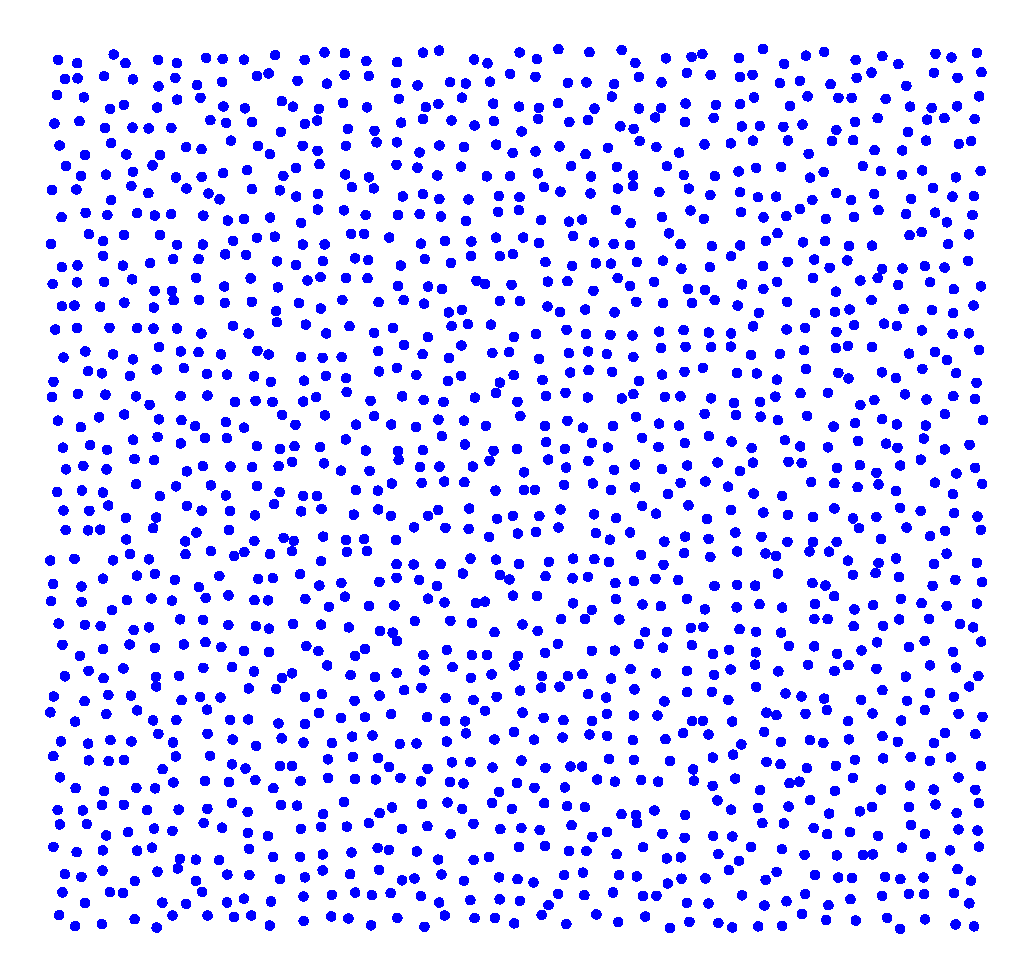
\includegraphics[width=0.90 \textwidth]{./Project1}
    \end{minipage}%
    \begin{minipage}{.325 \textwidth}
        \centering
        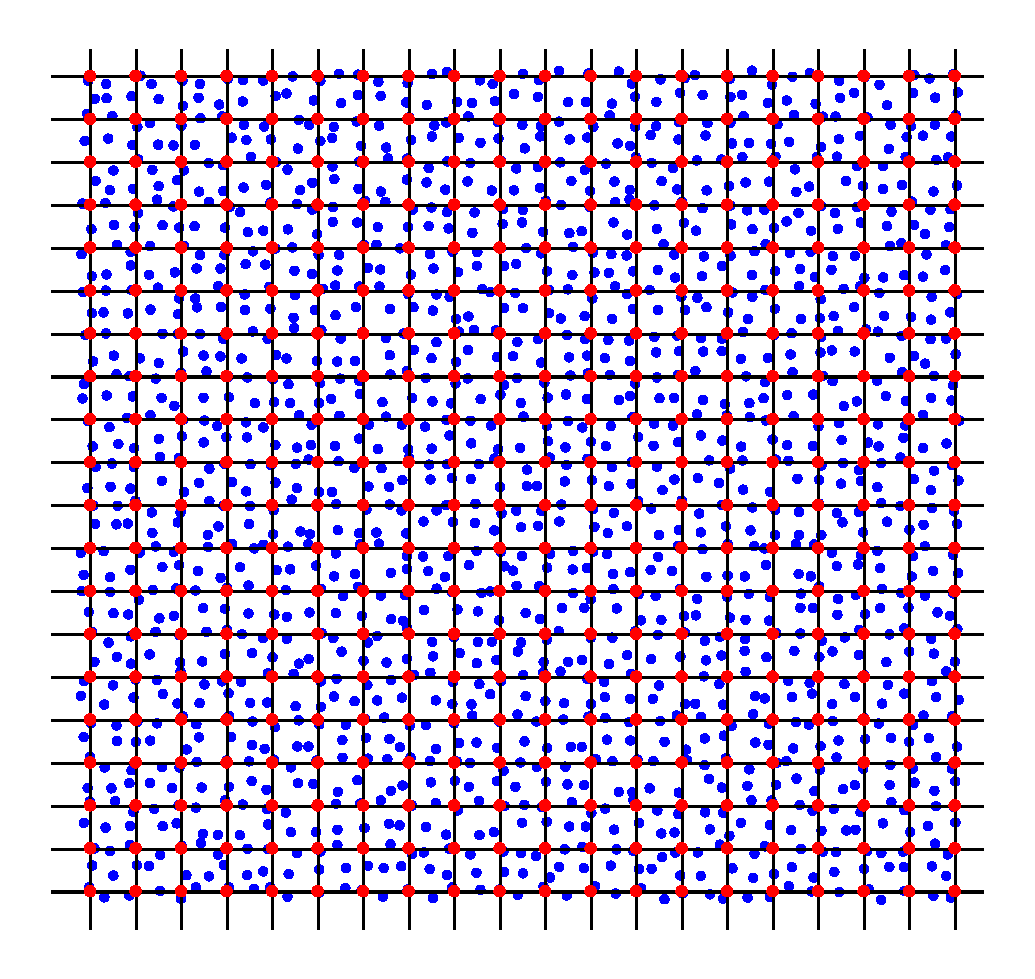
\includegraphics[width=0.90 \textwidth]{./Project2}
    \end{minipage}%
    \begin{minipage}{.325 \textwidth}
        \centering
        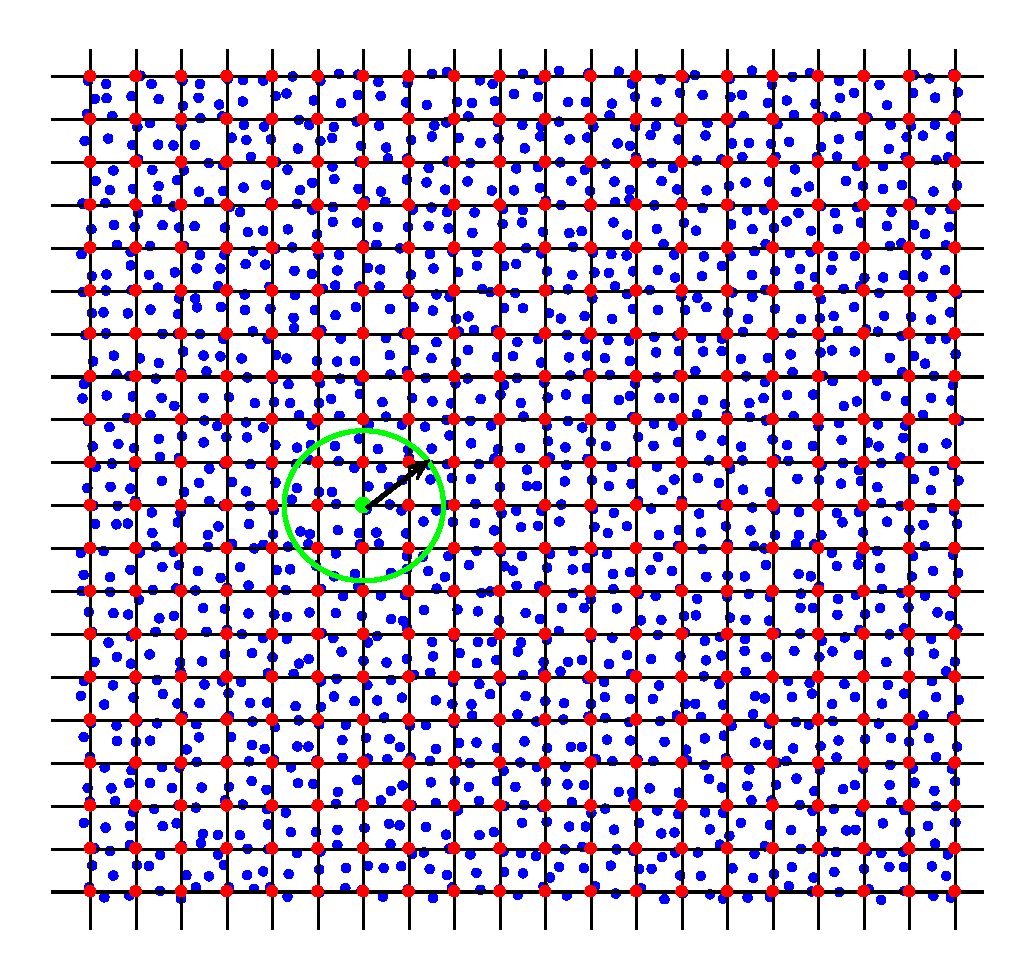
\includegraphics[width=0.90 \textwidth]{./Project3}
    \end{minipage}%   
    \caption{Procedure of projection of simulation results carried by particles onto regular grids. as shown in these figures from left to right: 1) raw data of SPH simulation results (irregularly distributed in space), 2) Add regular mesh, 3) searching for neighbours of each node (the blue SPH particles within the green circle around the red dot). The last step is not shown in these pictures, which is treating each node on the regular mesh as a SPH particle and projecting data on particles onto nodes utilizing "SPH interpolation" ( see Eq. (\ref{eq:SPH-fundamental-principle})).}
    \label{appfig:1D-shock-tests-verification}
\end{figure}

Particles distribute irregularly in SPH simulation results. To adapt post processing originally proposed for mesh-based method, we need to project simulation results onto a pre-defined regular mesh. As shown in Fig. \ref{appfig:1D-shock-tests-verification}, the basic steps for such projection are:
\begin{itemize}
\item obtain raw simulation results carried by particles that irregularly distribute in the space
\item create regular grids
\item search for neighbour paricles for each node of the regular grids.
\item interpolate physical quanties from neighbour particle onto corresponding node of regular grids according to Eq. (\ref{eq:SPH-fundamental-principle})
\end{itemize}

%
%\subsection{}     %% Appendix A1, A2, etc.
%
%\appendixfigures  %% needs to be added in front of appendix figures in one-column style (\documentclass[acp, manuscript]{copernicus})
%
%\appendixtables   %% needs to be added in front of appendix tables in one-column style (\documentclass[acp, manuscript]{copernicus})
%\authorcontribution{TEXT}

\competinginterests{Authors have the standard conflict with employers and listed sponsors}
%\disclaimer{TEXT}

\begin{acknowledgements}
All developers of Titan-2D, especially Dinesh Kumar who developed the GSPH version of Titan-2D, are greatly appreciated as Plume-SPH is based on their code. Advice and data (which is not shown in this paper) given by Suzuki Yujiro gave us great help at the initial stage of model establishment and therefor are greatly appreciated. We appreciate Tomaso Esposti Ongaro for providing simulation data of PDAC (were also provided by Antonio Costa later together with simulation results of other plume models) which helped us in doing early verification and improvement. We appreciate Antonio Costa for providing simulation results of existing 3D models, which are used in verification and validation section of this paper. We thank Matteo Cerminara for his helping on post-processing of plume simulation results. Computational results reported here were performed at the Center for Computational Research at the University at Buffalo. This project is supported by Grants No. NSF ACI/1131074 from the National Science Foundation.
\end{acknowledgements}

\clearpage

%% REFERENCES
%% The reference list is compiled as follows:
\bibliographystyle{copernicus}
\bibliography{Reference}
%% Since the Copernicus LaTeX package includes the BibTeX style file copernicus.bst,
%% authors experienced with BibTeX only have to include the following two lines:
%%
%% \bibliographystyle{copernicus}
%% \bibliography{example.bib}
%%
%% URLs and DOIs can be entered in your BibTeX file as:
%%
%% URL = {http://www.xyz.org/~jones/idx_g.htm}
%% DOI = {10.5194/xyz}
%% LITERATURE CITATIONS
%%
%% command                        & example result
%% \citet{jones90}|               & Jones et al. (1990)
%% \citep{jones90}|               & (Jones et al., 1990)
%% \citep{jones90,jones93}|       & (Jones et al., 1990, 1993)
%% \citep[p.~32]{jones90}|        & (Jones et al., 1990, p.~32)
%% \citep[e.g.,][]{jones90}|      & (e.g., Jones et al., 1990)
%% \citep[e.g.,][p.~32]{jones90}| & (e.g., Jones et al., 1990, p.~32)
%% \citeauthor{jones90}|          & Jones et al.
%% \citeyear{jones90}|            & 1990
%% FIGURES
%% When figures and tables are placed at the end of the MS (article in one-column style), please add \clearpage
%% between bibliography and first table and/or figure as well as between each table and/or figure.
%% ONE-COLUMN FIGURES
%%f
%\begin{figure}[t]
%\includegraphics[width=8.3cm]{FILE NAME}
%\caption{TEXT}
%\end{figure}
%
%%% TWO-COLUMN FIGURES
%
%%f
%\begin{figure*}[t]
%\includegraphics[width=12cm]{FILE NAME}
%\caption{TEXT}
%\end{figure*}
%
%
%%% TABLES
%%%
%%% The different columns must be seperated with a & command and should
%%% end with \\ to identify the column brake.
%
%%% ONE-COLUMN TABLE
%
%%t
%\begin{table}[t]
%\caption{TEXT}
%\begin{tabular}{column = lcr}
%\tophline
%
%\middlehline
%
%\bottomhline
%\end{tabular}
%\belowtable{} % Table Footnotes
%\end{table}
%
%%% TWO-COLUMN TABLE
%
%%t
%\begin{table*}[t]
%\caption{TEXT}
%\begin{tabular}{column = lcr}
%\tophline
%
%\middlehline
%
%\bottomhline
%\end{tabular}
%\belowtable{} % Table Footnotes
%\end{table*}
%
%
%%% MATHEMATICAL EXPRESSIONS
%
%%% All papers typeset by Copernicus Publications follow the math typesetting regulations
%%% given by the IUPAC Green Book (IUPAC: Quantities, Units and Symbols in Physical Chemistry,
%%% 2nd Edn., Blackwell Science, available at: http://old.iupac.org/publications/books/gbook/green_book_2ed.pdf, 1993).
%%%
%%% Physical quantities/variables are typeset in italic font (t for time, T for Temperature)
%%% Indices which are not defined are typeset in italic font (x, y, z, a, b, c)
%%% Items/objects which are defined are typeset in roman font (Car A, Car B)
%%% Descriptions/specifications which are defined by itself are typeset in roman font (abs, rel, ref, tot, net, ice)
%%% Abbreviations from 2 letters are typeset in roman font (RH, LAI)
%%% Vectors are identified in bold italic font using \vec{x}
%%% Matrices are identified in bold roman font
%%% Multiplication signs are typeset using the LaTeX commands \times (for vector products, grids, and exponential notations) or \cdot
%%% The character * should not be applied as mutliplication sign
%
%
%%% EQUATIONS
%
%%% Single-row equation
%
%\begin{equation}
%
%\end{equation}
%
%%% Multiline equation
%
%\begin{align}
%& 3 + 5 = 8\\
%& 3 + 5 = 8\\
%& 3 + 5 = 8
%\end{align}
%
%
%%% MATRICES
%
%\begin{matrix}
%x & y & z\\
%x & y & z\\
%x & y & z\\
%\end{matrix}
%
%
%%% ALGORITHM
%
%\begin{algorithm}
%\caption{_}
%\label{a1}
%\begin{algorithmic}
%_
%\end{algorithmic}
%\end{algorithm}
%
%
%%% CHEMICAL FORMULAS AND REACTIONS
%
%%% For formulas embedded in the text, please use \chem{}
%
%%% The reaction environment creates labels including the letter R, i.e. (R1), (R2), etc.
%
%\begin{reaction}
%%% \rightarrow should be used for normal (one-way) chemical reactions
%%% \rightleftharpoons should be used for equilibria
%%% \leftrightarrow should be used for resonance structures
%\end{reaction}
%
%
%%% PHYSICAL UNITS
%%%
%%% Please use \unit{} and apply the exponential notation
\end{document}
